\section{Графики решения}
1. $y=\cfrac{|x+1|}{x+1}(x-1)=\begin{cases} x-1,\ x>-1,\\ 1-x,\ x<-1.\end{cases}$
$$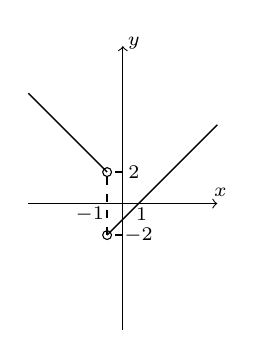
\begin{tikzpicture}[scale=0.2]
\tikzset {line01/.style={line width =0.5pt}}
\tikzset{line02/.style={line width =1pt}}
\tikzset{line03/.style={dashed,line width =0.5pt}}
%\filldraw [black] (0,0) circle (1pt);
\draw [->] (-6,0) -- (6,0);
\draw [->] (0,-8) -- (0,10);
\draw[line01] (-6,7) -- (-1,2);
\draw[line01] (-1,-2) -- (6,5);
\draw[line03] (-1,-2) -- (-1,2);
\draw[line03] (0,2) -- (-1,2);
\draw[line03] (0,-2) -- (-1,-2);
\draw (6.2,0.7) node {\scriptsize $x$};
\draw (1,-2) node {\scriptsize $-2$};
\draw (0.7,2) node {\scriptsize $2$};
\draw (1.2,-0.7) node {\scriptsize $1$};
\draw (-2.1,-0.7) node {\scriptsize $-1$};
\draw (0.7,10.2) node {\scriptsize $y$};
\draw (-1,2) circle (8pt);
\draw (-1,-2) circle (8pt);
\end{tikzpicture}$$
2. $y=\cfrac{|x-1|}{x-1}(x+1)=\begin{cases} x+1,\ x>1,\\ -x-1,\ x<1.\end{cases}$
$$\begin{tikzpicture}[scale=0.2]
\tikzset {line01/.style={line width =0.5pt}}
\tikzset{line02/.style={line width =1pt}}
\tikzset{line03/.style={dashed,line width =0.5pt}}
%\filldraw [black] (0,0) circle (1pt);
\draw [->] (-6,0) -- (6,0);
\draw [->] (0,-8) -- (0,10);
\draw[line01] (-6,5) -- (1,-2);
\draw[line01] (1,2) -- (6,7);
\draw[line03] (1,-2) -- (1,2);
\draw[line03] (0,2) -- (1,2);
\draw[line03] (0,-2) -- (1,-2);
\draw (6.2,0.7) node {\scriptsize $x$};
\draw (-1.2,-2) node {\scriptsize $-2$};
\draw (-0.7,2) node {\scriptsize $2$};
\draw (1.4,-0.7) node {\scriptsize $1$};
\draw (-2.1,-0.7) node {\scriptsize $-1$};
\draw (0.7,10.2) node {\scriptsize $y$};
\draw (1,2) circle (8pt);
\draw (1,-2) circle (8pt);
\end{tikzpicture}$$
3. $f(x)=\cfrac{|x^2-4x+3|}{|x-1|}=\cfrac{|x-1||x-3|}{|x-1|}=|x-3|,\ x
eq1.$
$$\begin{tikzpicture}[scale=0.2]
\tikzset {line01/.style={line width =0.5pt}}
\tikzset{line02/.style={line width =1pt}}
\tikzset{line03/.style={dashed,line width =0.5pt}}
%\filldraw [black] (0,0) circle (1pt);
\draw [->] (-5,0) -- (11,0);
\draw [->] (0,-8) -- (0,10);
\draw[line01] (-5,8) -- (3,0);
\draw[line01] (3,0) -- (11,8);
\draw[line03] (1,0) -- (1,2);
\draw[line03] (1,2) -- (0,2);
%\draw[line03] (1,-2) -- (0,-2);
\draw (11.2,0.7) node {\scriptsize $x$};
%\draw (-1.9,-1) node {\tiny $-1$};
%\draw (-1,-2) node {\scriptsize $-2$};
\draw (-0.5,2) node {\scriptsize $2$};
\draw (1,-0.7) node {\tiny $1$};
\draw (3,-0.7) node {\scriptsize $3$};
\draw (0.7,10.2) node {\scriptsize $y$};
%\draw (1,2) circle (8pt);
\draw (1,2) circle (8pt);
\end{tikzpicture}$$
4. $f(x)=\cfrac{|x^2-x-2|}{|x+1|}=\cfrac{|x+1||x-2|}{|x+1|}=|x-2|,\ x
eq-1.$
$$\begin{tikzpicture}[scale=0.2]
\tikzset {line01/.style={line width =0.5pt}}
\tikzset{line02/.style={line width =1pt}}
\tikzset{line03/.style={dashed,line width =0.5pt}}
%\filldraw [black] (0,0) circle (1pt);
\draw [->] (-5,0) -- (11,0);
\draw [->] (0,-8) -- (0,10);
\draw[line01] (-5,7) -- (2,0);
\draw[line01] (2,0) -- (9,7);
\draw[line03] (-1,0) -- (-1,3);
\draw[line03] (-1,3) -- (0,3);
%\draw[line03] (1,-2) -- (0,-2);
\draw (11.2,0.7) node {\scriptsize $x$};
\draw (-1.5,-1) node {\tiny $-1$};
%\draw (-1,-2) node {\scriptsize $-2$};
\draw (0.5,3) node {\scriptsize $3$};
%\draw (1,-0.7) node {\tiny $1$};
\draw (2,-0.7) node {\scriptsize $2$};
\draw (0.7,10.2) node {\scriptsize $y$};
%\draw (1,2) circle (8pt);
\draw (-1,3) circle (8pt);
\end{tikzpicture}$$
5. $f(x)=\cfrac{|x^2-4x|}{x}+|-x|=\cfrac{|x||x-4|}{x}+|x|=\begin{cases} 2x-4,\ x\geqslant4,\\ 4,\ 0<x<4,\\ -4,\ x<0.\end{cases}$
$$\begin{tikzpicture}[scale=0.2]
\tikzset {line01/.style={line width =0.5pt}}
\tikzset{line02/.style={line width =1pt}}
\tikzset{line03/.style={dashed,line width =0.5pt}}
%\filldraw [black] (0,0) circle (1pt);
\draw [->] (-5,0) -- (11,0);
\draw [->] (0,-8) -- (0,10);
\draw[line01] (-5,-4) -- (0,-4);
\draw[line01] (0,4) -- (4,4);
\draw[line01] (4,4) -- (7,10);
\draw[line03] (4,0) -- (4,4);
\draw[line03] (5,0) -- (5,6);
\draw[line03] (0,6) -- (5,6);
%\draw[line03] (-1,3) -- (0,3);
%\draw[line03] (1,-2) -- (0,-2);
\draw (11.2,0.7) node {\scriptsize $x$};
\draw (5,-1) node {\scriptsize $5$};
\draw (1,-4) node {\scriptsize $-4$};
\draw (-1,4) node {\scriptsize $4$};
\draw (-1,6) node {\scriptsize $6$};
%\draw (1,-0.7) node {\tiny $1$};
\draw (4,-1) node {\scriptsize $4$};
\draw (0.7,10.2) node {\scriptsize $y$};
%\draw (1,2) circle (8pt);
\draw (0,-4) circle (8pt);
\draw (0,4) circle (8pt);
\end{tikzpicture}$$
6. $f(x)=\cfrac{|x^2-2x|}{x-2}+|x|=\cfrac{|x||x-2|}{x-2}+|x|=\begin{cases} 2x,\ x>2,\\ 0,\ x<2.\end{cases}$
$$\begin{tikzpicture}[scale=0.2]
\tikzset {line01/.style={line width =0.5pt}}
\tikzset{line02/.style={line width =1pt}}
\tikzset{line03/.style={dashed,line width =0.5pt}}
%\filldraw [black] (0,0) circle (1pt);
\draw [->] (-5,0) -- (11,0);
\draw [->] (0,-8) -- (0,10);
\draw[line02] (-5,0) -- (1.9,0);
\draw[line02] (2,4) -- (5,10);
%\draw[line01] (4,4) -- (7,10);
\draw[line03] (2,0) -- (2,4);
\draw[line03] (2,4) -- (0,4);
\draw[line03] (4,0) -- (4,8);
\draw[line03] (0,8) -- (4,8);
%\draw[line03] (-1,3) -- (0,3);
%\draw[line03] (1,-2) -- (0,-2);
\draw (11.2,0.7) node {\scriptsize $x$};
%\draw (5,-1) node {\scriptsize $5$};
\draw (2,-1) node {\scriptsize $2$};
\draw (-1,4) node {\scriptsize $4$};
\draw (-1,8) node {\scriptsize $8$};
%\draw (1,-0.7) node {\tiny $1$};
\draw (4,-1) node {\scriptsize $4$};
\draw (0.7,10.2) node {\scriptsize $y$};
%\draw (1,2) circle (8pt);
\draw (2,0) circle (8pt);
\draw (2,4) circle (8pt);
\end{tikzpicture}$$
7. По теореме Виета $x_1+x_2=4,\ x_1x_2=\cfrac{q}{2}.$ Тогда $x_1^2+x_2^2=(x_1+x_2)^2-2x_1x_2=16-q=10,\ q=6.$ Параболу $2x^2-8x+6$ построим по трём точкам $(3;0),\ (1;0),\ (2;-2).$
$$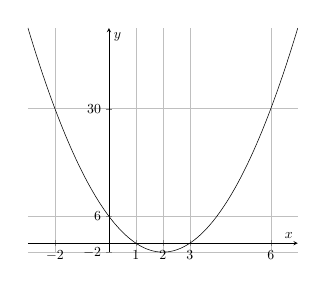
\begin{tikzpicture}[scale=0.5]
\begin{axis}[
    axis lines = middle,
    grid=major,
    legend pos={south west},
    xlabel = {$x$},
    %xlabel style={below right},
    ylabel = {$y$},
    xtick={-2, 1,2, 3, 6},
    ytick={-2,6,30},
               ]
	\addplot[domain=-3:7, samples=100, color=black] {2*x*x-8*x+6};
%\addplot[domain=-3.1:2.5, samples=100, color=red] {70*abs(1-2*abs(abs(x)-2))-10*x^2+10*x-70};
	%\addlegendentry{$\text{Рис. 1}$};
\end{axis}
\end{tikzpicture}$$
8. По теореме Виета $x_1+x_2=1,\ x_1x_2=-\cfrac{q}{2}.$ Тогда $(x_1-x_2)^2=(x_1+x_2)^2-4x_1x_2=1+2q=9,\ q=4.$ Параболу $-2x^2+2x+4$ построим по трём точкам $(2;0),\ (-1;0),\ \left(\cfrac{1}{2};\cfrac{9}{2}
ight).$
$$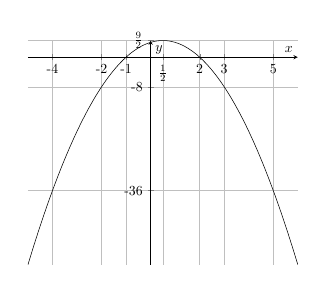
\begin{tikzpicture}[scale=0.5]
\begin{axis}[
    axis lines = middle,
    grid=major,
    legend pos={south west},
    xlabel = {$x$},
    %xlabel style={below right},
    ylabel = {$y$},
    xtick={-4, -2,-1,0.5,2, 3, 5},
    xticklabels={-4, -2,-1,$\frac{1}{2}$,2, 3,5},
    ytick={-36,-8,4.5},
    yticklabels={-36,-8,$\frac{9}{2}$},
               ]
	\addplot[domain=-5:6, samples=100, color=black] {-2*x*x+2*x+4};
%\addplot[domain=-3.1:2.5, samples=100, color=red] {70*abs(1-2*abs(abs(x)-2))-10*x^2+10*x-70};
	%\addlegendentry{$\text{Рис. 1}$};
\end{axis}
\end{tikzpicture}$$
9. $y=\cfrac{x+1}{x}=1+\cfrac{1}{x}.$ Центр симметрии этого графика находится в точке пересечения асимптот $x=0$ и $y=1,$ то есть в точке $(0;1).$ Действительно, если $f(x)=1+\cfrac{1}{x},$ то $f(0+x)+f(0-x)=1+\cfrac{1}{x}+1-\cfrac{1}{x}=2=2\cdot1.$\\
10. $y=\cfrac{1-x}{x}=-1+\cfrac{1}{x}.$ Центр симметрии этого графика находится в точке пересечения асимптот $x=0$ и $y=-1,$ то есть в точке $(0;-1).$ Действительно, если $f(x)=-1+\cfrac{1}{x},$ то $f(0+x)+f(0-x)=-1+\cfrac{1}{x}-1-\cfrac{1}{x}=-2=2\cdot(-1).$\\
11. Прямая $3y+4x=12$ пересекает начало координат $O$ в точках $A(3;0)$ и $B(0;4).$ Треугольник $OAB$ является прямоугольным и расстояние от начала координат до прямой $3y+4x=12$ равно его высоте, опущенной на гипотенузу. Длина гипотенузы равна $\sqrt{3^2+4^2}=5,$ поэтому $S_{\Delta OAB}=\cfrac{1}{2}\cdot4\cdot3=\cfrac{1}{2}\cdot h\cdot5,$ откуда $h=\cfrac{12}{5}.$\\
12. Прямая $3y-4x=12$ пересекает начало координат $O$ в точках $A(-3;0)$ и $B(0;4).$ Треугольник $OAB$ является прямоугольным и расстояние от начала координат до прямой $3y-4x=12$ равно его высоте, опущенной на гипотенузу. Длина гипотенузы равна $\sqrt{3^2+4^2}=5,$ поэтому $S_{\Delta OAB}=\cfrac{1}{2}\cdot4\cdot3=\cfrac{1}{2}\cdot h\cdot5,$ откуда $h=\cfrac{12}{5}.$\\
13. $y=|x+1|+|x+3|=\begin{cases}-2x-4,\ x<-3,\\ 2,\ -3\leqslant x\leqslant -1,\\ 2x+4,\ x>-1.\end{cases}$ Осью симметрии этого графика является вертикальная прямая, делящая пополам отрезок $[-3;-1],$ то есть $x=-2.$ Действительно, $|-2+x+1|+|-2+x+3|=|x-1|+|x+1|=|-2-x+3|+|-2-x+1|.$\\
14. $y=|x-1|+|x-3|=\begin{cases}-2x+4,\ x<1,\\ 2,\ 1\leqslant x\leqslant 3,\\ 2x-4,\ x>3.\end{cases}$ Осью симметрии этого графика является вертикальная прямая, делящая пополам отрезок $[1;3],$ то есть $x=2.$ Действительно, $|2-x-1|+|2-x-3|=|x-1|+|x+1|=|2+x-3|+|2+x-1|.$\\
15. $x^2+y^2-4x-6y=0\Leftrightarrow (x-2)^2+(y-3)^2=13.$ Значит, центр окружности находится в точке $(2;3),$ а радиус равен $\sqrt{13}.$\\
16. $x^2+y^2+6x-4y+2=0\Leftrightarrow (x+3)^2+(y-2)^2=11.$ Значит, центр окружности находится в точке $(-3;2),$ а радиус равен $\sqrt{11}.$\\
17. $y=\cfrac{|x-2|}{2-x}(x^2-2x)=\begin{cases}2x-x^2,\ x>2,\\ x^2-2x,\ x<2.\end{cases}$
$$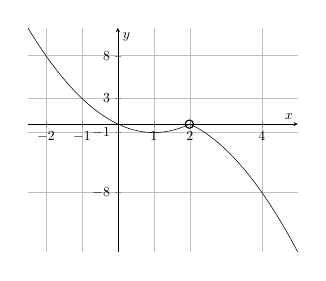
\begin{tikzpicture}[scale=0.5]
\begin{axis}[
    axis lines = middle,
    grid=major,
    legend pos={south west},
    xlabel = {$x$},
    %xlabel style={below right},
    ylabel = {$y$},
    xtick={-2, -1,1, 2,4},
    ytick={8,3,-1,-8},
                  ]
	\addplot[domain=-2.5:2, samples=100, color=black] {x*x-2*x};
    \addplot[domain=2:5, samples=100, color=black] {-x*x+2*x};
	%\addlegendentry{$\text{Рис. 1}$};
\end{axis}
\draw (4.1,3.25) circle (3pt);
\end{tikzpicture}$$
18. $y=\cfrac{|x+2|}{2+x}(x^2+4x+3)=\begin{cases}x^2+4x+3,\ x>-2,\\ -x^2-4x-3,\ x<-2.\end{cases}$
$$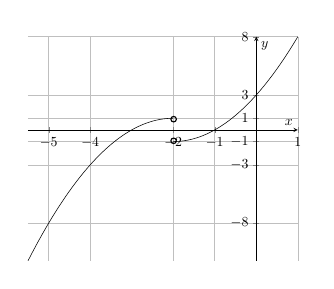
\begin{tikzpicture}[scale=0.5]
\begin{axis}[
    axis lines = middle,
    grid=major,
    legend pos={south west},
    xlabel = {$x$},
    %xlabel style={below right},
    ylabel = {$y$},
    xtick={-5,-4,-2, -1,1},
    ytick={-8, -3, 1, -1,8,3},
                  ]
	\addplot[domain=-5.5:-2, samples=100, color=black] {-x*x-4*x-3};
    \addplot[domain=-2:1, samples=100, color=black] {x*x+4*x+3};
	%\addlegendentry{$\text{Рис. 1}$};
\end{axis}
\draw (3.7,3.6) circle (2pt);
\draw (3.7,3.05) circle (2pt);
\end{tikzpicture}$$
19. $y=\cfrac{x^2+7x+6}{x+|x+2|}=\begin{cases}\cfrac{(x+6)(x+1)}{2x+2},\ x\geqslant-2,\\ \cfrac{(x+6)(x+1)}{-2},\ x<-2.\end{cases}=
\begin{cases}\cfrac{x+6}{2},\ x\geqslant-2,\ x
eq-1,\\ -\cfrac{1}{2}x^2-\cfrac{7}{2}x-3,\ x<-2.\end{cases}$
$$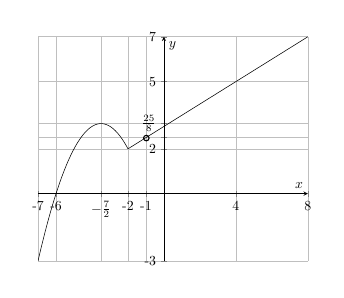
\begin{tikzpicture}[scale=0.5]
\begin{axis}[
    axis lines = middle,
    grid=major,
    legend pos={south west},
    xlabel = {$x$},
    %xlabel style={below right},
    ylabel = {$y$},
    xtick={-7, -6, -3.5,-2,-1, 4,8},
    xticklabels={-7, -6, $-\frac{7}{2}$,-2,-1, 4,8},
    ytick={-3, 3.125,2,2.5, 5,7},
    yticklabels={-3,$\frac{25}{8}$,2,$ $,5,7},
                  ]
	\addplot[domain=-7:-2, samples=100, color=black] {(x*x+7*x+6)/(-2)};
    \addplot[domain=-2:8, samples=100, color=black] {(x+6)/2};
	%\addlegendentry{$\text{Рис. 1}$};
\end{axis}
\draw (2.75,3.12) circle (2pt);
%\draw (3.7,3.05) circle (2pt);
\end{tikzpicture}$$
20. $y=\cfrac{x^2-6x+5}{x-|x-2|}=\begin{cases}\cfrac{(x-5)(x-1)}{2},\ x\geqslant2,\\ \cfrac{(x-5)(x-1)}{2x-2},\ x<2,\ x
eq1.\end{cases}=
\begin{cases}\cfrac{1}{2}x^2-3x+\cfrac{5}{2},\ x\geqslant2,\\ \cfrac{x-5}{2},\ x<2,\ x
eq1.\end{cases}$
$$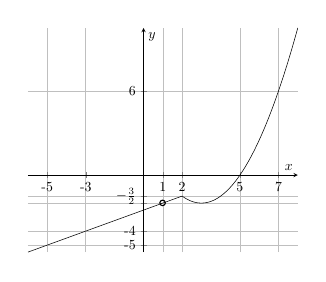
\begin{tikzpicture}[scale=0.5]
\begin{axis}[
    axis lines = middle,
    grid=major,
    legend pos={south west},
    xlabel = {$x$},
    %xlabel style={below right},
    ylabel = {$y$},
    xtick={-5, -3,1, 2,5,7},
    xticklabels={-5, -3,1, 2,5,7},
    ytick={-5,-4,-2,-1.5,6},
    yticklabels={-5,-4,$ $,$-\frac{3}{2}$,6},
                  ]
	\addplot[domain=-6:2, samples=100, color=black] {(x-5)/(2)};
    \addplot[domain=2:8, samples=100, color=black] {(x*x-6*x+5)/2};
	%\addlegendentry{$\text{Рис. 1}$};
\end{axis}
\draw (3.42,1.25) circle (2pt);
%\draw (3.7,3.05) circle (2pt);
\end{tikzpicture}$$
21. Так как ветви параболы направлены вверх, $a>0.$ Так как $x_{\text{верш}}=-\cfrac{b}{2a}>0,$ то $b<0.$ Так как значение параболы при $x=0$ отрицательно, $c<0.$\\
22. Так как ветви параболы направлены вниз, $a<0.$ Так как $x_{\text{верш}}=-\cfrac{b}{2a}>0,$ то $b>0.$ Так как значение параболы при $x=0$ отрицательно, $c<0.$\\
23. $y=\cfrac{\sqrt{(x+1)^2-4x}}{x^2-x}=\cfrac{\sqrt{(x-1)^2}}{x(x-1)}=\cfrac{|x-1|}{x(x-1)}=\begin{cases}\cfrac{1}{x},\ x>1,\\ -\cfrac{1}{x},\ x<1\end{cases}.$
$$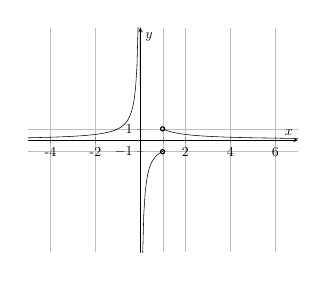
\begin{tikzpicture}[scale=0.5]
\begin{axis}[
    axis lines = middle,
    grid=major,
    legend pos={south west},
    xlabel = {$x$},
    %xlabel style={below right},
    ylabel = {$y$},
    ymin=-10,
    ymax=10,
    xtick={-4, -2,1,2,4,6},
    xticklabels={-4, -2,$ $,2, 4,6},
    ytick={1,-1},
    %yticklabels={-5,-4,$ $,$-\frac{3}{2}$,6},
                  ]
	\addplot[domain=-5:1, samples=100, color=black] {-1/x};
    \addplot[domain=1:7, samples=100, color=black] {1/x};
	%\addlegendentry{$\text{Рис. 1}$};
\end{axis}
\draw (3.42,2.55) circle (1.5pt);
\draw (3.42,3.13) circle (1.5pt);
%\draw (3.7,3.05) circle (2pt);
\end{tikzpicture}$$
24. $y=\cfrac{\sqrt{(x-1)^2+4x}}{x^2+x}=\cfrac{\sqrt{(x+1)^2}}{x(x+1)}=\cfrac{|x+1|}{x(x+1)}=\begin{cases}\cfrac{1}{x},\ x>-1,\\ -\cfrac{1}{x},\ x<-1\end{cases}.$
$$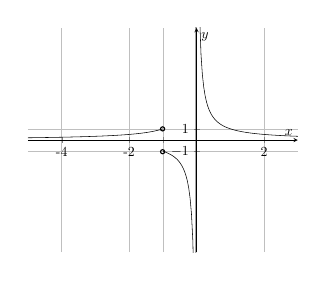
\begin{tikzpicture}[scale=0.5]
\begin{axis}[
    axis lines = middle,
    grid=major,
    legend pos={south west},
    xlabel = {$x$},
    %xlabel style={below right},
    ylabel = {$y$},
    ymin=-10,
    ymax=10,
    xtick={-4, -2,-1,2,4,6},
    xticklabels={-4, -2,$ $,2, 4,6},
    ytick={1,-1},
    %yticklabels={-5,-4,$ $,$-\frac{3}{2}$,6},
                  ]
	\addplot[domain=-5:-1, samples=100, color=black] {-1/x};
    \addplot[domain=-1:3, samples=100, color=black] {1/x};
	%\addlegendentry{$\text{Рис. 1}$};
\end{axis}
\draw (3.42,2.55) circle (1.5pt);
\draw (3.42,3.13) circle (1.5pt);
%\draw (3.7,3.05) circle (2pt);
\end{tikzpicture}$$
25. $(|y|-3)(y+|x|-1)=0\Leftrightarrow \left[\begin{array}{l} |y|-3=0,\\ y+|x|-1=0.\end{array}
ight.\Leftrightarrow\left[\begin{array}{l} y=3,\\ y=-3,\\ y=1-|x|.\end{array}
ight.$
$$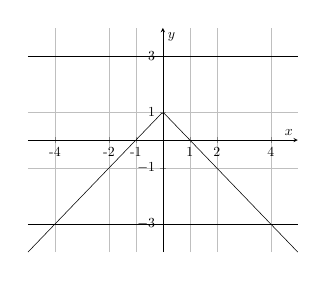
\begin{tikzpicture}[scale=0.5]
\begin{axis}[
    axis lines = middle,
    grid=major,
    legend pos={south west},
    xlabel = {$x$},
    %xlabel style={below right},
    ylabel = {$y$},
    ymin=-4,
    ymax=4,
    xtick={-4, -2,-1,1, 2,4},
    xticklabels={-4, -2,-1,1, 2, 4},
    ytick={1,-1,-3,3},
     %yticklabels={-5,-4,$ $,$-\frac{3}{2}$,6},
                  ]
	\addplot[domain=-5:5, samples=100, color=black] {3};
    \addplot[domain=-5:5, samples=100, color=black] {-3};
    \addplot[domain=-5:5, samples=100, color=black] {1-abs(x)};
	%\addlegendentry{$\text{Рис. 1}$};
\end{axis}
%\draw (3.7,3.05) circle (2pt);
\end{tikzpicture}$$
26. $(|x|-3)(x+|y|-1)=0\Leftrightarrow \left[\begin{array}{l} |x|-3=0,\\ x+|y|-1=0.\end{array}
ight.\Leftrightarrow\left[\begin{array}{l} x=3,\\ x=-3,\\ y=1-x,\ x\leqslant1,\\ y=x-1,\ x \leqslant1.\end{array}
ight.$
$$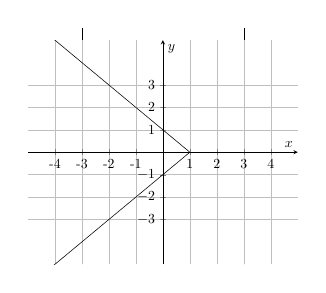
\begin{tikzpicture}[scale=0.5]
\tikzset {line01/.style={line width =0.3pt}}
\draw[line01] (1.38,0) -- (1.38,6);
\draw[line01] (5.5,0) -- (5.5,6);
\begin{axis}[
    axis lines = middle,
    grid=major,
    legend pos={south west},
    xlabel = {$x$},
    %xlabel style={below right},
    ylabel = {$y$},
    xmin=-5,
    xmax=5,
    ymin=-5,
    ymax=5,
    xtick={-4, -3, -2,-1,1, 2,3,4},
    xticklabels={-4,-3, -2,-1,1, 2,3, 4},
    ytick={1,-1,-3,3,-2,2},
     %yticklabels={-5,-4,$ $,$-\frac{3}{2}$,6},
                  ]
	\addplot[domain=-5:1, samples=100, color=black] {1-x};
    \addplot[domain=-5:1, samples=100, color=black] {x-1};

	%\addlegendentry{$\text{Рис. 1}$};
\end{axis}
%\draw (3.7,3.05) circle (2pt);
\end{tikzpicture}$$
27. а) $f(x)=\cfrac{x-2+|2x-1|}{x^2-1}=\begin{cases}\cfrac{3x-3}{(x-1)(x+1)},\ x\geqslant\cfrac{1}{2},\\ \cfrac{-x-1}{(x-1)(x+1)},\ x<\cfrac{1}{2}.\end{cases}=
\begin{cases}\cfrac{3}{x+1},\ x\geqslant\cfrac{1}{2},\ x
eq1,\\ \cfrac{1}{1-x},\ x<\cfrac{1}{2},\ x
eq-1.\end{cases}$
$$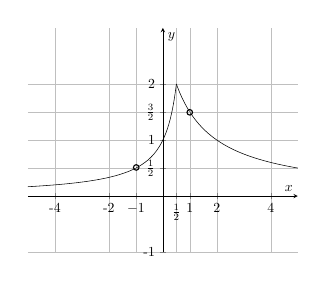
\begin{tikzpicture}[scale=0.5]
\begin{axis}[
    axis lines = middle,
    grid=major,
    legend pos={south west},
    xlabel = {$x$},
    %xlabel style={below right},
    ylabel = {$y$},
    ymin=-1,
    ymax=3,
    xtick={-4, -2,-1,0.5,1, 2,4},
    xticklabels={-4, -2,$-1$,$\frac{1}{2}$, 1, 2, 4},
    ytick={-1,0.5, 1, 1.5, 2},
     yticklabels={-1,$\frac{1}{2}$, 1, $\frac{3}{2}$, 2},
                  ]
	\addplot[domain=-5:-1.01, samples=100, color=black] {1/(1-x)};
    \addplot[domain=-0.99:0.5, samples=100, color=black] {1/(1-x)};
    \addplot[domain=0.5:0.99, samples=100, color=black] {3/(x+1)};
    \addplot[domain=1.01:5, samples=100, color=black] {3/(x+1)};
    %\addlegendentry{$\text{Рис. 1}$};
\end{axis}
\draw (2.75,2.15) circle (2pt);
\draw (4.11,3.55) circle (2pt);
\end{tikzpicture}$$
б) По графику определим $D(f)=(-\infty;-1)\cup(-1;1)\cup(1;+\infty),\ E(f)=(0;2].$\\
в) По графику определим количесво решений: $a\in(-\infty;0]\cup(2;+\infty):0,\ a\in\left\{\cfrac{1}{2}; \cfrac{3}{2},2
ight\}:1,\ a\in\left(0;\cfrac{1}{2}
ight)\cup\left(\cfrac{1}{2};\cfrac{3}{2}
ight)\cup\left(\cfrac{3}{2};2
ight):2.$\\
28. $f(x)=\cfrac{x+2-|2x+1|}{x^2-1}=\begin{cases}\cfrac{-x+1}{(x-1)(x+1)},\ x\geqslant-\cfrac{1}{2},\\ \cfrac{3x+3}{(x-1)(x+1)},\ x<-\cfrac{1}{2}.\end{cases}=
\begin{cases}-\cfrac{1}{x+1},\ x\geqslant-\cfrac{1}{2},\ x
eq1,\\ \cfrac{3}{x-1},\ x<-\cfrac{1}{2},\ x
eq-1.\end{cases}$
$$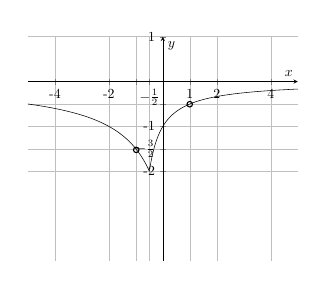
\begin{tikzpicture}[scale=0.5]
\begin{axis}[
    axis lines = middle,
    grid=major,
    legend pos={south west},
    xlabel = {$x$},
    %xlabel style={below right},
    ylabel = {$y$},
    ymin=-4,
    ymax=1,
    xtick={-4, -2,-1,-0.5,1, 2,4},
    xticklabels={-4, -2,$ $,$-\frac{1}{2}$, 1, 2, 4},
    ytick={-2,-1.5,-1,-0.5, 1, 2},
     yticklabels={-2,$-\frac{3}{2}$,-1,$ $, 1, 2},
                  ]
	\addplot[domain=-5:-0.5, samples=100, color=black] {3/(x-1)};
    %\addplot[domain=-0.99:0.5, samples=100, color=black] {1/(1-x)};
    \addplot[domain=-0.5:5, samples=100, color=black] {-1/(x+1)};
   % \addplot[domain=1.01:5, samples=100, color=black] {3/(x+1)};
    %\addlegendentry{$\text{Рис. 1}$};
\end{axis}
\draw (2.75,2.82) circle (2pt);
\draw (4.11,3.98) circle (2pt);
\end{tikzpicture}$$
б) По графику определим $D(f)=(-\infty;-1)\cup(-1;1)\cup(1;+\infty),\ E(f)=[-2;0).$\\
в) По графику определим количесво решений: $a\in(-\infty;-2)\cup[0;+\infty):0,\ a\in\left\{-2;-\cfrac{3}{2}; -\cfrac{1}{2}
ight\}:1,$\\$ a\in\left(-2;-\cfrac{3}{2}
ight)\cup\left(-\cfrac{3}{2};-\cfrac{1}{2}
ight)\cup\left(-\cfrac{1}{2};0
ight):2.$\\
29. $\cfrac{x^2+y^2-9}{x^2-y^2}=0\Leftrightarrow \begin{cases}x^2+y^2-9=0,\\ x^2-y^2
eq0.\end{cases}
\Leftrightarrow \begin{cases}x^2+y^2=3^2,\\ y
eq x,\\ y
eq -x.\end{cases}$
$$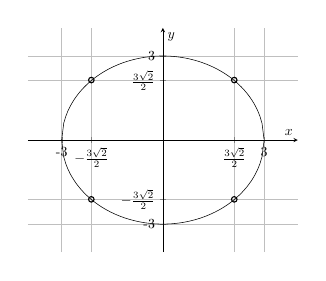
\begin{tikzpicture}[scale=0.5]
\begin{axis}[
    axis lines = middle,
    grid=major,
    legend pos={south west},
    xlabel = {$x$},
    %xlabel style={below right},
    ylabel = {$y$},
    ymin=-4,
    ymax=4,
    xmin=-4,
    xmax=4,
    xtick={-3,-2.12,2.12,3},
    xticklabels={-3,$-\frac{3\sqrt{2}}{2}$,$\frac{3\sqrt{2}}{2}$,3},
    ytick={-3,-2.12,2.12,3},
    yticklabels={-3,$-\frac{3\sqrt{2}}{2}$,$\frac{3\sqrt{2}}{2}$,3},
                  ]
	\addplot[domain=-3:3, samples=100, color=black] {sqrt(9-x*x)};
    \addplot[domain=-3:3, samples=100, color=black] {-sqrt(9-x*x)};
     %\addlegendentry{$\text{Рис. 1}$};
\end{axis}
\draw (5.24,4.37) circle (2pt);
\draw (1.61,4.37) circle (2pt);
\draw (1.61,1.34) circle (2pt);
\draw (5.24,1.34) circle (2pt);
\end{tikzpicture}$$
30. $\cfrac{x^2+y^2-1}{x^2-y^2}=0\Leftrightarrow \begin{cases}x^2+y^2-1=0,\\ x^2-y^2
eq0.\end{cases}
\Leftrightarrow \begin{cases}x^2+y^2=1^2,\\ y
eq x,\\ y
eq -x.\end{cases}$
$$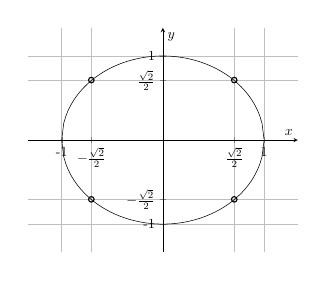
\begin{tikzpicture}[scale=0.5]
\begin{axis}[
    axis lines = middle,
    grid=major,
    legend pos={south west},
    xlabel = {$x$},
    %xlabel style={below right},
    ylabel = {$y$},
    ymin=-4,
    ymax=4,
    xmin=-4,
    xmax=4,
    xtick={-3,-2.12,2.12,3},
    xticklabels={-1,$-\frac{\sqrt{2}}{2}$,$\frac{\sqrt{2}}{2}$,1},
    ytick={-3,-2.12,2.12,3},
    yticklabels={-1,$-\frac{\sqrt{2}}{2}$,$\frac{\sqrt{2}}{2}$,1},
                  ]
	\addplot[domain=-3:3, samples=100, color=black] {sqrt(9-x*x)};
    \addplot[domain=-3:3, samples=100, color=black] {-sqrt(9-x*x)};
     %\addlegendentry{$\text{Рис. 1}$};
\end{axis}
\draw (5.24,4.37) circle (2pt);
\draw (1.61,4.37) circle (2pt);
\draw (1.61,1.34) circle (2pt);
\draw (5.24,1.34) circle (2pt);
\end{tikzpicture}$$
31. $y=\cfrac{x-2}{|x^2-2x|}=\cfrac{x-2}{|x||x-2|}=\begin{cases} \cfrac{1}{x},\ x>2,\\ -\cfrac{1}{x},\ 0<x<2,\\ \cfrac{1}{x},\ x<0. \end{cases}$
$$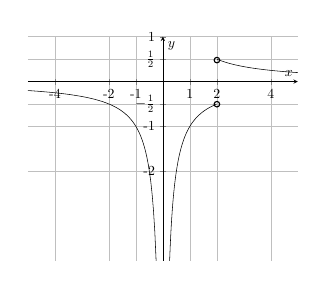
\begin{tikzpicture}[scale=0.5]
\begin{axis}[
    axis lines = middle,
    grid=major,
    legend pos={south west},
    xlabel = {$x$},
    %xlabel style={below right},
    ylabel = {$y$},
    ymin=-4,
    ymax=1,
    xtick={-4, -2,-1,1, 2,4},
    xticklabels={-4, -2,-1, 1, 2, 4},
    ytick={-2,-1,-0.5,0.5, 1, 2},
     yticklabels={-2,-1,$-\frac{1}{2}$,$\frac{1}{2}$, 1, 2},
                  ]
	\addplot[domain=-5:-0.1, samples=100, color=black] {1/x};
    \addplot[domain=0.1:1.99, samples=100, color=black] {-1/x};
    \addplot[domain=2.01:5, samples=100, color=black] {1/x};
   % \addplot[domain=1.01:5, samples=100, color=black] {3/(x+1)};
    %\addlegendentry{$\text{Рис. 1}$};
\end{axis}
\draw (4.8,5.1) circle (2pt);
\draw (4.8,3.98) circle (2pt);
\end{tikzpicture}$$
32. $y=\cfrac{3-x}{|x^2-3x|}=\cfrac{3-x}{|x||x-3|}=\begin{cases} -\cfrac{1}{x},\ x>3,\\ \cfrac{1}{x},\ 0<x<3,\\ -\cfrac{1}{x},\ x<0. \end{cases}$
$$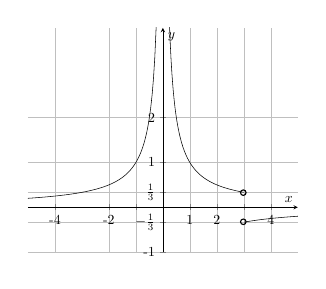
\begin{tikzpicture}[scale=0.5]
\begin{axis}[
    axis lines = middle,
    grid=major,
    legend pos={south west},
    xlabel = {$x$},
    %xlabel style={below right},
    ylabel = {$y$},
    ymin=-1,
    ymax=4,
    xtick={-4, -2,-1,1, 2,3,4},
    xticklabels={-4, -2,$ $, 1, 2,$ $, 4},
    ytick={-2,-1,-0.33,0.33, 1, 2},
     yticklabels={-2,-1,$-\frac{1}{3}$,$\frac{1}{3}$, 1, 2},
                  ]
	\addplot[domain=-5:-0.1, samples=100, color=black] {-1/x};
    \addplot[domain=0.1:2.99, samples=100, color=black] {1/x};
    \addplot[domain=3.01:5, samples=100, color=black] {-1/x};
   % \addplot[domain=1.01:5, samples=100, color=black] {3/(x+1)};
    %\addlegendentry{$\text{Рис. 1}$};
\end{axis}
\draw (5.47,1.51) circle (2pt);
\draw (5.47,0.77) circle (2pt);
\end{tikzpicture}$$
33. Прямая $y=1-\cfrac{x}{2}$ образует с осями координат прямоугольный треугольник $O(0;0),\ A(0;1),$\\$ B(2;0),$ его гипотенуза равна $AB=\sqrt{1^2+2^2}=\sqrt{5}.$ Расстояние от начала координат до этой прямоу равно высоте $h,$ проведённой к его гипотенузе. Найдём его площадь двумя способами: $S_{\Delta OAB}=\cfrac{1}{2}\cdot1\cdot2=\cfrac{1}{2}\cdot h\cdot\sqrt{5},$ откуда $h=\cfrac{2}{\sqrt{5}}=\cfrac{2\sqrt{5}}{5}.$\\
34. Прямая $y=2-2x$ образует с осями координат прямоугольный треугольник $O(0;0),\ A(0;2),$\\$ B(1;0),$ его гипотенуза равна $AB=\sqrt{2^2+1^2}=\sqrt{5}.$ Расстояние от начала координат до этой прямоу равно высоте $h,$ проведённой к его гипотенузе. Найдём его площадь двумя способами: $S_{\Delta OAB}=\cfrac{1}{2}\cdot2\cdot1=\cfrac{1}{2}\cdot h\cdot\sqrt{5},$ откуда $h=\cfrac{2}{\sqrt{5}}=\cfrac{2\sqrt{5}}{5}.$\\
35. Пусть искомая функция имеет вид $f(x)=ax^2+bx+c.$ Подставим точку $A:\ 0+0+c=-2,\ c=-2.$ Единственное значение парабола принимает только в вершине, исходя из этого составим систему уравнений:
$\begin{cases} 4a-2b-2=4,\\ a\cdot\cfrac{b^2}{4a^2}-b\cdot\cfrac{b}{2a}-2=-4.\end{cases}\Leftrightarrow
\begin{cases} b=2a-3,\\ \cfrac{-b^2}{4a}=-2.\end{cases}\Leftrightarrow
\begin{cases} b=2a-3,\\ (2a-3)^2=8a.\end{cases}\Leftrightarrow
\begin{cases} b=2a-3,\\ 4a^2-20a+9=0.\end{cases}\Leftrightarrow
\left[\begin{array}{l}\begin{cases} a=\cfrac{1}{2},\\ b=-2.\end{cases}\\\begin{cases} a=\cfrac{9}{2},\\ b=6.\end{cases}\end{array}
ight.$\\
Таким образом, искомая функция равна $\frac{1}{2}x^2-2x-2$ или $\frac{9}{2}x^2+6x-2.$\\
36. Пусть искомая функция имеет вид $f(x)=ax^2+bx+c.$ У квадратичной функции совпадают значения, симметричные относительно вершины, значит $-\cfrac{b}{2a}=\cfrac{-1+2}{2}=\cfrac{1}{2},\ b=-a.$ Наибольшее значение квадратичной функции достигается в вершине (при это должно выполняться неравенство $a<0).$ Исходя из этого, составим систему уравнений (второе уравнение получим из того, что парабола проходит через точку $(1;1))$: $\begin{cases}
a\cdot\cfrac{1}{4}-a\cdot\cfrac{1}{2}+c=3,\\ a-a+c=1.\end{cases}\Leftrightarrow
\begin{cases}
a=-8,\\ c=1.\end{cases}$\\
Таким образом, искомая функция равна $-8x^2+8x+1.$\\
37. а) $f(x)=\cfrac{x-1+|x-1|}{x^2-1}=\begin{cases}\cfrac{2x-2}{(x-1)(x+1)},\ x>1,\\ 0,\ x<1,\ x
eq-1.\end{cases}=
\begin{cases}\cfrac{2}{x+1},\ x>1,\\ 0,\ x<1,\ x
eq-1.\end{cases}$
$$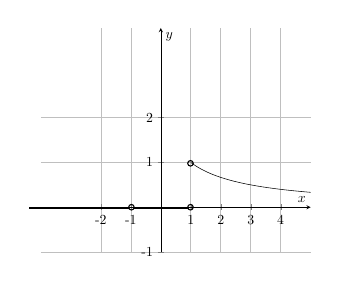
\begin{tikzpicture}[scale=0.5]
\tikzset {line01/.style={line width =0.5pt}}
\tikzset{line02/.style={line width =1pt}}
\tikzset{line03/.style={dashed,line width =0.5pt}}
\begin{axis}[
    axis lines = middle,
    grid=major,
    legend pos={south west},
    xlabel = {$x$},
    %xlabel style={below right},
    ylabel = {$y$},
    xmin=-4,
    ymin=-1,
    ymax=4,
    xtick={-2,-1,1, 2,3,4},
    xticklabels={-2,-1,1, 2,3,4},
    ytick={-1, 1, 2},
    yticklabels={-1, 1, 2},
                  ]
	%\addplot[domain=-5:0.99, samples=100, color=black] {0};
    \addplot[domain=1:5, samples=100, color=black] {2/(x+1)};
    %\addplot[domain=3.01:5, samples=100, color=black] {-1/x};
   % \addplot[domain=1.01:5, samples=100, color=black] {3/(x+1)};
    %\addlegendentry{$\text{Рис. 1}$};
\end{axis}
\draw (3.8,2.255) circle (2pt);
\draw (3.8,1.14) circle (2pt);
\draw (2.3,1.14) circle (2pt);
\draw[line02] (-0.3,1.12) -- (2.25,1.12);
\draw[line02] (2.35,1.12) -- (3.75,1.12);
\end{tikzpicture}$$
б) По графику определим $D(f)=(-\infty;-1)\cup(-1;1)\cup(1;+\infty).$\\
в) По графику определим количество решений: $a\in(-\infty;0)\cup[1;+\infty):0,\ a\in(0;1): 1,\ a=0:\infty.$\\
38. $f(x)=\cfrac{x+1-|x+1|}{x^2-1}=\begin{cases}\cfrac{2x+2}{(x-1)(x+1)},\ x<-1,\\ 0,\ x>-1,\ x
eq1.\end{cases}=
\begin{cases}\cfrac{2}{x-1},\ x<-1,\\ 0,\ x>-1,\ x
eq1.\end{cases}$
$$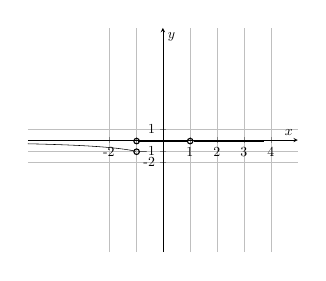
\begin{tikzpicture}[scale=0.5]
\tikzset {line01/.style={line width =0.5pt}}
\tikzset{line02/.style={line width =1pt}}
\tikzset{line03/.style={dashed,line width =0.5pt}}
\begin{axis}[
    axis lines = middle,
    grid=major,
    legend pos={south west},
    xlabel = {$x$},
    %xlabel style={below right},
    ylabel = {$y$},
    xmin=-5,
    xmax=5,
    ymin=-10,
    ymax=10,
    xtick={-2,-1,1, 2,3,4},
    xticklabels={-2,$ $,1, 2,3,4},
    ytick={-2, -1, 1},
    yticklabels={-2, $-1$, 1},
                  ]
	%\addplot[domain=-5:0.99, samples=100, color=black] {0};
    \addplot[domain=-5:-1, samples=100, color=black] {2/(x-1)};
    %\addplot[domain=1.01:5, samples=100, color=black] {2/(x-1)};
    %\addplot[domain=3.01:5, samples=100, color=black] {-1/x};
   % \addplot[domain=1.01:5, samples=100, color=black] {3/(x+1)};
    %\addlegendentry{$\text{Рис. 1}$};
\end{axis}
%\draw (3.8,2.255) circle (2pt);
%\draw (3.8,1.14) circle (2pt);
\draw (2.76,2.82) circle (2pt);
\draw (2.76,2.55) circle (2pt);
\draw (4.12,2.82) circle (2pt);
\draw[line02] (2.8,2.82) -- (4.06,2.82);
\draw[line02] (4.22,2.82) -- (6,2.82);
%\draw[line02] (2.35,1.1) -- (3.75,1.1);
\end{tikzpicture}$$
б) По графику определим $D(f)=(-\infty;-1)\cup(-1;1)\cup(1;+\infty).$\\
в) По графику определим количество решений: $a\in(-\infty;-1]\cup(0;+\infty):0,\ a\in(-1;0): 1,\ a=0:\infty.$\\
39. $\cfrac{x^2-y^2}{x^2+y^2-9}=0\Leftrightarrow \begin{cases} x^2-y^2=0,\\ x^2+y^2-9
eq0\end{cases}
\Leftrightarrow \begin{cases}\left[\begin{array}{l} y=x,\\ y=-x.\end{array}
ight.\\ x^2+y^2
eq3^2\end{cases}$
$$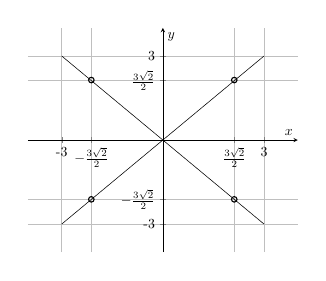
\begin{tikzpicture}[scale=0.5]
\begin{axis}[
    axis lines = middle,
    grid=major,
    legend pos={south west},
    xlabel = {$x$},
    %xlabel style={below right},
    ylabel = {$y$},
    ymin=-4,
    ymax=4,
    xmin=-4,
    xmax=4,
    xtick={-3,-2.12,2.12,3},
    xticklabels={-3,$-\frac{3\sqrt{2}}{2}$,$\frac{3\sqrt{2}}{2}$,3},
    ytick={-3,-2.12,2.12,3},
    yticklabels={-3,$-\frac{3\sqrt{2}}{2}$,$\frac{3\sqrt{2}}{2}$,3},
                  ]
	\addplot[domain=-3:3, samples=100, color=black] {x};
    \addplot[domain=-3:3, samples=100, color=black] {-x};
     %\addlegendentry{$\text{Рис. 1}$};
\end{axis}
\draw (5.24,4.37) circle (2pt);
\draw (1.61,4.37) circle (2pt);
\draw (1.61,1.34) circle (2pt);
\draw (5.24,1.34) circle (2pt);
\end{tikzpicture}$$
40. $\cfrac{x^2-y^2}{x^2+y^2-1}=0\Leftrightarrow \begin{cases} x^2-y^2=0,\\ x^2+y^2-1
eq0\end{cases}
\Leftrightarrow \begin{cases}\left[\begin{array}{l} y=x,\\ y=-x.\end{array}
ight.\\ x^2+y^2
eq1^2\end{cases}$
$$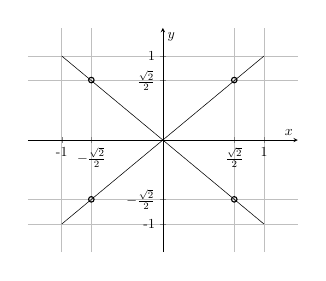
\begin{tikzpicture}[scale=0.5]
\begin{axis}[
    axis lines = middle,
    grid=major,
    legend pos={south west},
    xlabel = {$x$},
    %xlabel style={below right},
    ylabel = {$y$},
    ymin=-4,
    ymax=4,
    xmin=-4,
    xmax=4,
    xtick={-3,-2.12,2.12,3},
    xticklabels={-1,$-\frac{\sqrt{2}}{2}$,$\frac{\sqrt{2}}{2}$,1},
    ytick={-3,-2.12,2.12,3},
    yticklabels={-1,$-\frac{\sqrt{2}}{2}$,$\frac{\sqrt{2}}{2}$,1},
                  ]
	\addplot[domain=-3:3, samples=100, color=black] {x};
    \addplot[domain=-3:3, samples=100, color=black] {-x};
     %\addlegendentry{$\text{Рис. 1}$};
\end{axis}
\draw (5.24,4.37) circle (2pt);
\draw (1.61,4.37) circle (2pt);
\draw (1.61,1.34) circle (2pt);
\draw (5.24,1.34) circle (2pt);
\end{tikzpicture}$$
41. $\cfrac{x^2-y^2}{x^2+y^2-4}=0\Leftrightarrow \begin{cases} x^2-y^2=0,\\ x^2+y^2-4
eq0\end{cases}
\Leftrightarrow \begin{cases}\left[\begin{array}{l} y=x,\\ y=-x.\end{array}
ight.\\ x^2+y^2
eq2^2\end{cases}$
$$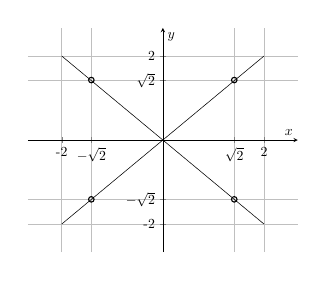
\begin{tikzpicture}[scale=0.5]
\begin{axis}[
    axis lines = middle,
    grid=major,
    legend pos={south west},
    xlabel = {$x$},
    %xlabel style={below right},
    ylabel = {$y$},
    ymin=-4,
    ymax=4,
    xmin=-4,
    xmax=4,
    xtick={-3,-2.12,2.12,3},
    xticklabels={-2,$-\sqrt{2}$,$\sqrt{2}$,2},
    ytick={-3,-2.12,2.12,3},
    yticklabels={-2,$-\sqrt{2}$,$\sqrt{2}$,2},
                  ]
	\addplot[domain=-3:3, samples=100, color=black] {x};
    \addplot[domain=-3:3, samples=100, color=black] {-x};
     %\addlegendentry{$\text{Рис. 1}$};
\end{axis}
\draw (5.24,4.37) circle (2pt);
\draw (1.61,4.37) circle (2pt);
\draw (1.61,1.34) circle (2pt);
\draw (5.24,1.34) circle (2pt);
\end{tikzpicture}$$
42. $\cfrac{x^2-y^2}{x^2+y^2-16}=0\Leftrightarrow \begin{cases} x^2-y^2=0,\\ x^2+y^2-16
eq0\end{cases}
\Leftrightarrow \begin{cases}\left[\begin{array}{l} y=x,\\ y=-x.\end{array}
ight.\\ x^2+y^2
eq4^2\end{cases}$
$$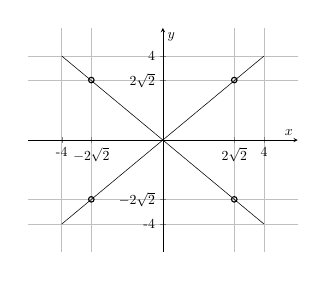
\begin{tikzpicture}[scale=0.5]
\begin{axis}[
    axis lines = middle,
    grid=major,
    legend pos={south west},
    xlabel = {$x$},
    %xlabel style={below right},
    ylabel = {$y$},
    ymin=-4,
    ymax=4,
    xmin=-4,
    xmax=4,
    xtick={-3,-2.12,2.12,3},
    xticklabels={-4,$-2\sqrt{2}$,$2\sqrt{2}$,4},
    ytick={-3,-2.12,2.12,3},
    yticklabels={-4,$-2\sqrt{2}$,$2\sqrt{2}$,4},
                  ]
	\addplot[domain=-3:3, samples=100, color=black] {x};
    \addplot[domain=-3:3, samples=100, color=black] {-x};
     %\addlegendentry{$\text{Рис. 1}$};
\end{axis}
\draw (5.24,4.37) circle (2pt);
\draw (1.61,4.37) circle (2pt);
\draw (1.61,1.34) circle (2pt);
\draw (5.24,1.34) circle (2pt);
\end{tikzpicture}$$
43. а) $f(x)=|x^2-2x|=\begin{cases} x^2-2x,\ x\leqslant 0,\\ 2x-x^2,\ 0<x<2,\\ x^2-2x,\ x\geqslant2.\end{cases}$
$$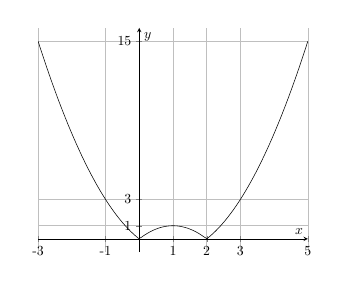
\begin{tikzpicture}[scale=0.5]
\begin{axis}[
    axis lines = middle,
    grid=major,
    legend pos={south west},
    xlabel = {$x$},
    %xlabel style={below right},
    ylabel = {$y$},
    ymin=-1,
    ymax=16,
    xmin=-3,
    xmax=5,
    xtick={-3,-1,1,2,3,5,7},
    xticklabels={-3,-1,1,2,3,5,7},
    ytick={ 15,3,1},
    yticklabels={ 15,3,1},
                  ]
	\addplot[domain=-3:5, samples=100, color=black] {abs(x*x-2*x)};
   % \addplot[domain=-3:3, samples=100, color=black] {-x};
     %\addlegendentry{$\text{Рис. 1}$};
\end{axis}
\end{tikzpicture}$$
б) По графику определим количество решений: $a\in(-\infty;0):0,\ a\in\{0\}\cup(1;+\infty):2,\ a=1: 3,$\\$ a\in(0;1): 4.$\\
44. $f(x)=|x^2+2x|=\begin{cases} x^2+2x,\ x\leqslant -2,\\ -2x-x^2,\ -2<x<0,\\ x^2+2x,\ x\geqslant0.\end{cases}$
$$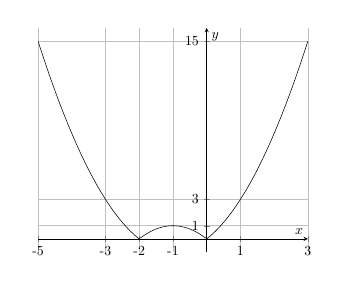
\begin{tikzpicture}[scale=0.5]
\begin{axis}[
    axis lines = middle,
    grid=major,
    legend pos={south west},
    xlabel = {$x$},
    %xlabel style={below right},
    ylabel = {$y$},
    ymin=-1,
    ymax=16,
    xmin=-5,
    xmax=3,
    xtick={3,1,-1,-2,-3,-5,-7},
    xticklabels={3,1,-1,-2,-3,-5,-7},
    ytick={ 15,3,1},
    yticklabels={ 15,3,1},
                  ]
	\addplot[domain=-5:3, samples=100, color=black] {abs(x*x+2*x)};
   % \addplot[domain=-3:3, samples=100, color=black] {-x};
     %\addlegendentry{$\text{Рис. 1}$};
\end{axis}
\end{tikzpicture}$$
б) По графику определим количество решений: $a\in(-\infty;0):0,\ a\in\{0\}\cup(1;+\infty):2,\ a=1: 3,$\\$ a\in(0;1): 4.$\\
45. $\cfrac{yx-x^2-y+1}{x-1}=0\Leftrightarrow \cfrac{y(x-1)-(x-1)(x+1)}{x-1}=0\Leftrightarrow \cfrac{(x-1)(y-x-1)}{x-1}=0
\Leftrightarrow y=x+1,\ x
eq1.$
$$\begin{tikzpicture}[scale=0.2]
\tikzset {line01/.style={line width =0.5pt}}
\tikzset{line02/.style={line width =1pt}}
\tikzset{line03/.style={dashed,line width =0.5pt}}
%\filldraw [black] (0,0) circle (1pt);
\draw [->] (-6,0) -- (6,0);
\draw [->] (0,-8) -- (0,10);
\draw[line01] (-6,-5) -- (6,7);
%\draw[line01] (-2,-7) -- (-2,7);
\draw[line03] (1,0) -- (1,2);
\draw[line03] (0,2) -- (1,2);
%\draw[line03] (0,-2) -- (1,-2);
\draw (6.2,0.7) node {\scriptsize $x$};
%\draw (-1.2,-2) node {\scriptsize $-2$};
%\draw (-0.7,2) node {\scriptsize $2$};
\draw (-0.7,2) node {\scriptsize $2$};
\draw (-0.7,1) node {\scriptsize $1$};
%\draw (0.7,-1) node {\tiny $-1$};
\draw (1,-0.7) node {\scriptsize $1$};
%\draw (-2.8,-0.9) node {\tiny $-2$};
\draw (0.7,10.2) node {\scriptsize $y$};
\draw (1,2) circle (8pt);
%\draw (-2,-3) circle (8pt);
\end{tikzpicture}$$
46. $\cfrac{(y-2x+1)(y+2x-1)}{y^2-x^2}=0\Leftrightarrow \begin{cases}\left[\begin{array}{l} y=2x-1,\\ y=1-2x.\end{array}
ight.\\ y
eq x,\\ y
eq-x.\end{cases}$
$$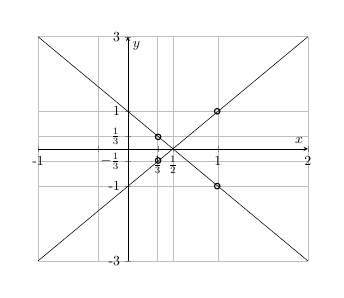
\begin{tikzpicture}[scale=0.5]
\begin{axis}[
    axis lines = middle,
    grid=major,
    legend pos={south west},
    xlabel = {$x$},
    %xlabel style={below right},
    ylabel = {$y$},
    ymin=-3,
    ymax=3,
    xmin=-1,
    xmax=2,
    xtick={-1,-0.33,0.33,0.5,1, 2},
    xticklabels={-1, $ $, $\frac{1}{3}$,$\frac{1}{2}$,1, 2},
    ytick={-3,-1,-0.33,0.33,1,3},
    yticklabels={-3,-1, $-\frac{1}{3}$,$\frac{1}{3}$,1,3},
                  ]
	\addplot[domain=-1:2, samples=100, color=black] {2*x-1};
    \addplot[domain=-1:2, samples=100, color=black] {-2*x+1};
   % \addplot[domain=-3:3, samples=100, color=black] {-x};
     %\addlegendentry{$\text{Рис. 1}$};
\end{axis}
\draw (4.55,3.8) circle (2pt);
\draw (3.05,3.15) circle (2pt);
\draw (3.05,2.55) circle (2pt);
\draw (4.55,1.9) circle (2pt);
\end{tikzpicture}$$
47. Пусть прямая $a$ имеет уравнение $y=kx+b,$ тогда $\begin{cases}b=4,\\6a+4=0.\end{cases}\Rightarrow y=-\cfrac{2}{3}x+4.$ Если прямая $b$ параллельна прямой $a,$ то она имеет уравнение $y=-\cfrac{2}{3}x+b_1,$ при этом $0+b_1=8,\ b_1=8.$ Тогда если $y=0,$ то $-\cfrac{2}{3}x+8=0,\ x=12.$\\
48. Пусть прямая $a$ имеет уравнение $y=kx+b,$ тогда $\begin{cases}b=4,\\-6a+4=0.\end{cases}\Rightarrow y=\cfrac{2}{3}x+4.$ Если прямая $b$ параллельна прямой $a,$ то она имеет уравнение $y=\cfrac{2}{3}x+b_1,$ при этом $0+b_1=-6,\ b_1=-6.$ Тогда если $y=0,$ то $\cfrac{2}{3}x-6=0,\ x=9.$\\
49. Так как обе функции при больших положительных значениях $x$ принимают положительные значения, при этом наклон $l_1$ <<круче>>, имеем $k_1>k_2>0.$
Так как прямая $l_1$ пересекает ось $y$ ниже, имеем $b_1<b_2<0.$ Таким образом, $b_1<b_2<k_2<k_1.$\\
50. Так как обе функции при больших положительных значениях $x$ принимают отрицательные значения, при этом наклон $l_1$ <<круче>>, имеем $k_1<k_2<0.$
Так как прямая $l_2$ пересекает ось $y$ выше, имеем $b_2>b_1>0.$ Таким образом, $k_1<k_2<b_1<b_2.$\\
51. а) $y=-|x^2-2x|=\begin{cases} 2x-x^2,\ x\leqslant0,\\ x^2-2x,\ 0<x<2,\\ 2x-x^2.\ x\geqslant2.\end{cases}$
$$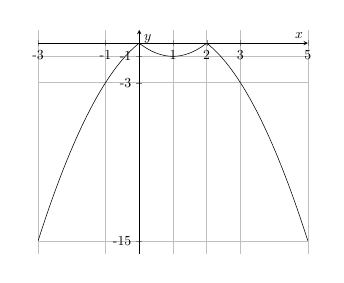
\begin{tikzpicture}[scale=0.5]
\begin{axis}[
    axis lines = middle,
    grid=major,
    legend pos={south west},
    xlabel = {$x$},
    %xlabel style={below right},
    ylabel = {$y$},
    ymin=-16,
    ymax=1,
    xmin=-3,
    xmax=5,
    xtick={-3,-1,1,2,3,5},
    xticklabels={-3,-1,1,2,3,5},
    ytick={ -15,-3,-1},
    yticklabels={ -15,-3,-1},
                  ]
	\addplot[domain=-3:5, samples=100, color=black] {-abs(x*x-2*x)};
   % \addplot[domain=-3:3, samples=100, color=black] {-x};
     %\addlegendentry{$\text{Рис. 1}$};
\end{axis}
\end{tikzpicture}$$
б) По графику найдём $a\in(-\infty;-1)\cup\{0\}.$\\
52. $y=|x^2-4x|=\begin{cases} x^2-4x,\ x\leqslant0,\\ 4x-x^2,\ 0<x<4,\\ x^2-4x.\ x\geqslant4.\end{cases}$
$$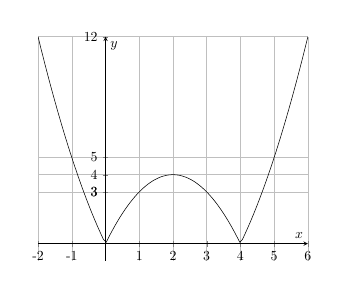
\begin{tikzpicture}[scale=0.5]
\begin{axis}[
    axis lines = middle,
    grid=major,
    legend pos={south west},
    xlabel = {$x$},
    %xlabel style={below right},
    ylabel = {$y$},
    ymin=-1,
    ymax=12,
    xmin=-2,
    xmax=6,
    xtick={-2,-1,1,2,3,4,5,6},
    xticklabels={-2,-1,1,2,3,4,5,6},
    ytick={5,3,12,3,4},
    yticklabels={5,3,12,3,4},
                  ]
	\addplot[domain=-2:6, samples=100, color=black] {abs(x*x-4*x)};
   % \addplot[domain=-3:3, samples=100, color=black] {-x};
     %\addlegendentry{$\text{Рис. 1}$};
\end{axis}
\end{tikzpicture}$$
б) По графику найдём $a\in\{0\}\cup(4;+\infty).$\\
53. Составим уравнение для нахождения общей точки: $(x+a)^2+1=4+2x,\ x^2+2(a-1)x+a^2-3=0.$ Это уравнение имеет одно решение, если $\cfrac{D}{4}=(a-1)^2-a^2+3=
a^2-2a+1-a^2+3=4-2a=0,\ a=2.$\\
54. Составим уравнение для нахождения общей точки: $-(x-a)^2+4=2x-5,\ x^2-2(a-1)x+a^2-9=0.$ Это уравнение имеет одно решение, если $\cfrac{D}{4}=(a-1)^2-a^2+9=
a^2-2a+1-a^2+9=10-2a=0,\ a=5.$\\
55. $|xy|>1\Leftrightarrow|y|>\cfrac{1}{|x|}\Leftrightarrow \left[\begin{array}{l}\begin{cases} x>0,\\ y>\cfrac{1}{x}.\end{cases}\\
\begin{cases} x>0,\\ y<-\cfrac{1}{x}.\end{cases}\\\begin{cases} x<0,\\ y>-\cfrac{1}{x}.\end{cases}\\\begin{cases} x<0,\\ y<\cfrac{1}{x}.\end{cases}\end{array}
ight.$
$$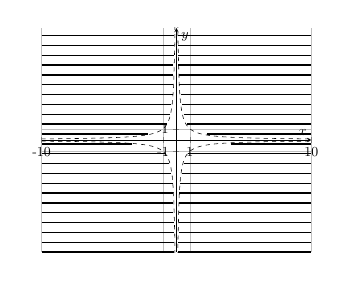
\begin{tikzpicture}[scale=0.5]
\tikzset {line01/.style={line width =0.5pt}}
\begin{axis}[
    axis lines = middle,
    grid=major,
    legend pos={south west},
    xlabel = {$x$},
    %xlabel style={below right},
    ylabel = {$y$},
    ymin=-10,
    ymax=10,
    xmin=-10,
    xmax=10,
    xtick={-10,-1,1,10},
    xticklabels={-10,-1,1,10},
    ytick={-1,1},
    yticklabels={$ $,1},
                  ]
	\addplot[dashed,domain=-10:-0.01, samples=100, color=black] {1/x};
    \addplot[dashed,domain=0.01:10, samples=100, color=black] {1/x};
    \addplot[dashed,domain=-10:-0.01, samples=100, color=black] {-1/x};
    \addplot[dashed,domain=0.01:10, samples=100, color=black] {-1/x};
   % \addplot[domain=-3:3, samples=100, color=black] {-x};
     %\addlegendentry{$\text{Рис. 1}$};
\end{axis}
\draw[line01] (0,0) -- (3.37,0);
\draw[line01] (0,0.25) -- (3.37,0.25);
\draw[line01] (0,0.5) -- (3.37,0.5);
\draw[line01] (0,0.75) -- (3.37,0.75);
\draw[line01] (0,1) -- (3.35,1);
\draw[line01] (0,1.25) -- (3.35,1.25);
\draw[line01] (0,1.5) -- (3.35,1.5);
\draw[line01] (0,1.75) -- (3.35,1.75);
\draw[line01] (0,2) -- (3.3,2);
\draw[line01] (0,2.25) -- (3.25,2.25);
\draw[line01] (0,2.5) -- (3.15,2.5);
\draw[line01] (0,2.75) -- (2.3,2.75);
\draw[line01] (0,3) -- (2.7,3);
\draw[line01] (0,3.25) -- (3.18,3.25);
\draw[line01] (0,3.5) -- (3.26,3.5);
\draw[line01] (0,3.75) -- (3.3,3.75);
\draw[line01] (0,4) -- (3.34,4);
\draw[line01] (0,4.25) -- (3.35,4.25);
\draw[line01] (0,4.5) -- (3.35,4.5);
\draw[line01] (0,4.75) -- (3.35,4.75);
\draw[line01] (0,5) -- (3.37,5);
\draw[line01] (0,5.25) -- (3.37,5.25);
\draw[line01] (0,5.5) -- (3.372,5.5);
\draw[line01] (3.47,5.5) -- (6.85,5.5);

\draw[line01] (3.47,0) -- (6.85,0);
\draw[line01] (3.47,0.25) -- (6.85,0.25);
\draw[line01] (3.48,0.5) -- (6.85,0.5);
\draw[line01] (3.5,0.75) -- (6.85,0.75);
\draw[line01] (3.5,1) -- (6.85,1);
\draw[line01] (3.5,1.25) -- (6.85,1.25);
\draw[line01] (3.5,1.5) -- (6.85,1.5);
\draw[line01] (3.53,1.75) -- (6.85,1.75);
\draw[line01] (3.56,2) -- (6.85,2);
\draw[line01] (3.61,2.25) -- (6.85,2.25);
\draw[line01] (3.71,2.5) -- (6.85,2.5);
\draw[line01] (4.81,2.75) -- (6.85,2.75);

\draw[line01] (4.2,3) -- (6.85,3);
\draw[line01] (3.7,3.25) -- (6.85,3.25);
\draw[line01] (3.61,3.5) -- (6.85,3.5);
\draw[line01] (3.57,3.75) -- (6.85,3.75);
\draw[line01] (3.55,4) -- (6.85,4);
\draw[line01] (3.49,4.25) -- (6.85,4.25);
\draw[line01] (3.5,4.5) -- (6.85,4.5);
\draw[line01] (3.47,4.75) -- (6.85,4.75);
\draw[line01] (3.47,5) -- (6.85,5);
\draw[line01] (3.47,5.25) -- (6.85,5.25);
\end{tikzpicture}$$
56. $|xy|<1\Leftrightarrow \left[\begin{array}{l}\begin{cases} x>0,\\ -\cfrac{1}{x}<y<\cfrac{1}{x}.\end{cases}\\
\begin{cases} x<0,\\ \cfrac{1}{x}<y<-\cfrac{1}{x}.\end{cases}\\ x=0,\\ y=0.\end{array}
ight.$
$$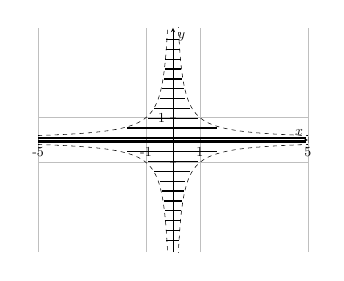
\begin{tikzpicture}[scale=0.5]
\tikzset {line01/.style={line width =0.5pt}}
\begin{axis}[
    axis lines = middle,
    grid=major,
    legend pos={south west},
    xlabel = {$x$},
    %xlabel style={below right},
    ylabel = {$y$},
    ymin=-5,
    ymax=5,
    xmin=-5,
    xmax=5,
    xtick={-5,-1,1,5},
    xticklabels={-5,-1,1,5},
    ytick={-1,1},
    yticklabels={$ $,1},
                  ]
	\addplot[dashed,domain=-5:-0.01, samples=100, color=black] {1/x};
    \addplot[dashed,domain=0.01:5, samples=100, color=black] {1/x};
    \addplot[dashed,domain=-5:-0.01, samples=100, color=black] {-1/x};
    \addplot[dashed,domain=0.01:5, samples=100, color=black] {-1/x};
   % \addplot[domain=-3:3, samples=100, color=black] {-x};
     %\addlegendentry{$\text{Рис. 1}$};
\end{axis}
\draw[line01] (0,2.8) -- (6.8,2.8);
\draw[line01] (0,2.9) -- (6.8,2.9);
\draw[line01] (2.26,3.15) -- (4.54,3.15);
\draw[line01] (2.8,3.4) -- (4.05,3.4);
\draw[line01] (2.95,3.65) -- (3.85,3.65);
\draw[line01] (3.1,3.9) -- (3.74,3.9);
\draw[line01] (3.15,4.15) -- (3.7,4.15);
\draw[line01] (3.2,4.4) -- (3.65,4.4);
\draw[line01] (3.22,4.65) -- (3.63,4.65);
\draw[line01] (3.22,4.9) -- (3.62,4.9);
\draw[line01] (3.24,5.15) -- (3.61,5.15);
\draw[line01] (3.26,5.4) -- (3.59,5.4);

\draw[line01] (2.26,2.55) -- (4.54,2.55);
\draw[line01] (2.8,2.3) -- (4.05,2.3);
\draw[line01] (2.95,2.05) -- (3.85,2.05);
\draw[line01] (3.1,1.8) -- (3.74,1.8);
\draw[line01] (3.15,1.55) -- (3.7,1.55);
\draw[line01] (3.2,1.3) -- (3.65,1.3);
\draw[line01] (3.22,1.05) -- (3.63,1.05);
\draw[line01] (3.22,0.8) -- (3.62,0.8);
\draw[line01] (3.24,0.55) -- (3.61,0.55);
\draw[line01] (3.26,0.3) -- (3.59,0.3);
\end{tikzpicture}$$
57. а) $y=-\cfrac{4(x+2)}{x^2+x-2}=-\cfrac{4(x+2)}{(x+2)(x-1)}=\cfrac{4}{1-x},\ x
eq-2.$
$$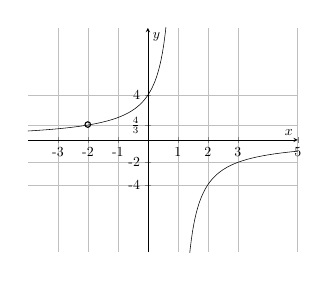
\begin{tikzpicture}[scale=0.5]
\begin{axis}[
    axis lines = middle,
    grid=major,
    legend pos={south west},
    xlabel = {$x$},
    %xlabel style={below right},
    ylabel = {$y$},
    ymin=-10,
    ymax=10,
    xmin=-4,
    xmax=5,
    xtick={-3,-2,-1,1,2,3,5},
    xticklabels={-3,-2,-1,1,2,3,5},
    ytick={-4,-2,1.333,4},
    yticklabels={-4,-2,$\frac{4}{3}$,4},
                  ]
	\addplot[domain=-4:0.99, samples=100, color=black] {4/(1-x)};
    \addplot[domain=1.01:5, samples=100, color=black] {4/(1-x)};
   % \addplot[domain=-3:3, samples=100, color=black] {-x};
     %\addlegendentry{$\text{Рис. 1}$};
\end{axis}
\draw (1.52,3.24) circle (2pt);
\end{tikzpicture}$$
б) По графику определим количество решений: $a\in\left\{0;\cfrac{4}{3}
ight\}:0,\ a\in(-\infty;0)\cup\left(0;\cfrac{4}{3}
ight)\cup\left(\cfrac{4}{3};+\infty
ight):1.$\\
58. а) $y=\cfrac{2(x-1)}{3x-2-x^2}=\cfrac{2(x-1)}{-(x-1)(x-2)}=\cfrac{2}{2-x},\ x
eq1.$
$$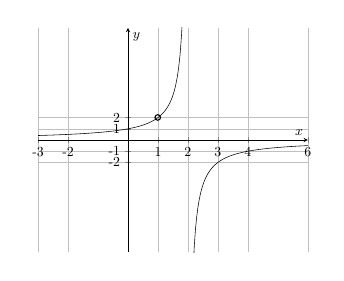
\begin{tikzpicture}[scale=0.5]
\begin{axis}[
    axis lines = middle,
    grid=major,
    legend pos={south west},
    xlabel = {$x$},
    %xlabel style={below right},
    ylabel = {$y$},
    ymin=-10,
    ymax=10,
    xmin=-3,
    xmax=6,
    xtick={-2,-3,1,2,3,4,6},
    xticklabels={-2,-3,1,2,3,4,6},
    ytick={-2,-1,1,2},
    yticklabels={-2,-1,1,2},
                  ]
	\addplot[domain=-3:1.99, samples=100, color=black] {2/(2-x)};
    \addplot[domain=2.01:6, samples=100, color=black] {2/(2-x)};
   % \addplot[domain=-3:3, samples=100, color=black] {-x};
     %\addlegendentry{$\text{Рис. 1}$};
\end{axis}
\draw (3.04,3.42) circle (2pt);
\end{tikzpicture}$$
б) По графику определим количество решений: $a\in\left\{0;2
ight\}:0,\ a\in(-\infty;0)\cup\left(0;2
ight)\cup\left(2;+\infty
ight):1.$\\
59. Если $x$ и $y$ целые числа, то выражение $2x+6y$ чётно и не может быть равно 9.\\
60. Если $x$ и $y$ целые числа, то выражение $4x+6y$ чётно и не может быть равно 7.\\
61. $f(x)=x^2-|2x-2|-1=\begin{cases} x^2-2x+1,\ x\geqslant1,\\ x^2+2x-3,\ x<1.\end{cases}$
$$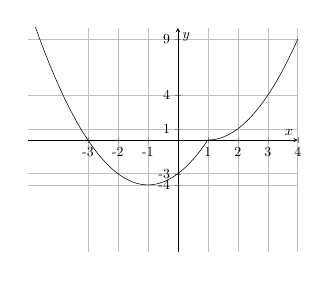
\begin{tikzpicture}[scale=0.5]
\begin{axis}[
    axis lines = middle,
    grid=major,
    legend pos={south west},
    xlabel = {$x$},
    %xlabel style={below right},
    ylabel = {$y$},
    ymin=-10,
    ymax=10,
    xmin=-5,
    xmax=4,
    xtick={-2,-3,-1,1,2,3,4,6},
    xticklabels={-2,-3,-1,1,2,3,4,6},
    ytick={-4,-3,1,4,9,25},
    yticklabels={-4,-3,1,4,9,25},
                  ]
	\addplot[domain=-5:4, samples=100, color=black] {x*x-abs(2*x-2)-1};
    %\addplot[domain=2.01:6, samples=100, color=black] {2/(2-x)};
   % \addplot[domain=-3:3, samples=100, color=black] {-x};
     %\addlegendentry{$\text{Рис. 1}$};
\end{axis}
%\draw (3.04,3.42) circle (2pt);
\end{tikzpicture}$$
По графику определим $E(f)=[-4;+\infty).$\\
62. $f(x)=(x+1)|x-1|=\begin{cases} x^2-1,\ x\geqslant1,\\ 1-x^2,\ x<1.\end{cases}$
$$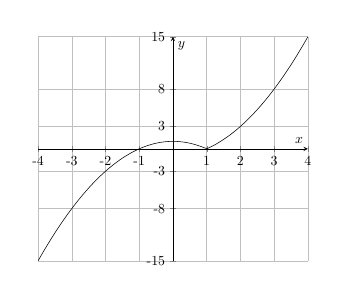
\begin{tikzpicture}[scale=0.5]
\begin{axis}[
    axis lines = middle,
    grid=major,
    legend pos={south west},
    xlabel = {$x$},
    %xlabel style={below right},
    ylabel = {$y$},
    ymin=-15,
    ymax=15,
    xmin=-4,
    xmax=4,
    xtick={-4,-2,-3,-1,1,2,3,4,6},
    xticklabels={-4,-2,-3,-1,1,2,3,4,6},
    ytick={-15,-3,-8,3,8,15},
    yticklabels={-15,-3,-8,3,8,15},
                  ]
	\addplot[domain=-4:4, samples=100, color=black] {(x+1)*abs(x-1)};
    %\addplot[domain=2.01:6, samples=100, color=black] {2/(2-x)};
   % \addplot[domain=-3:3, samples=100, color=black] {-x};
     %\addlegendentry{$\text{Рис. 1}$};
\end{axis}
%\draw (3.04,3.42) circle (2pt);
\end{tikzpicture}$$
По графику определим промежутки возрастания: $(-\infty;0]$ и $[1;+\infty).$\\
63. $y=\cfrac{(x^2+2x-8)(x+2)}{|x+2|}=\begin{cases} x^2+2x-8,\ x>-2,\\ -x^2-2x+8,\ x<-2.\end{cases}$
$$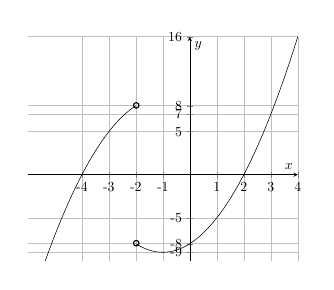
\begin{tikzpicture}[scale=0.5]
\begin{axis}[
    axis lines = middle,
    grid=major,
    legend pos={south west},
    xlabel = {$x$},
    %xlabel style={below right},
    ylabel = {$y$},
    ymin=-10,
    ymax=16,
    xmin=-6,
    xmax=4,
    xtick={-4,-2,-3,-1,1,2,3,4,6},
    xticklabels={-4,-2,-3,-1,1,2,3,4,6},
    ytick={-9,-8,-5,7,8,16,5},
    yticklabels={-9,-8,-5,7,8,16,5},
                  ]
	\addplot[domain=-6:-2, samples=100, color=black] {-(x*x+2*x-8)};
    \addplot[domain=-2:4, samples=100, color=black] {x*x+2*x-8};
    %\addplot[domain=2.01:6, samples=100, color=black] {2/(2-x)};
   % \addplot[domain=-3:3, samples=100, color=black] {-x};
     %\addlegendentry{$\text{Рис. 1}$};
\end{axis}
\draw (2.75,3.95) circle (2pt);
\draw (2.75,0.45) circle (2pt);
\end{tikzpicture}$$
По графику найдём $m\in(-9;-8).$\\
64. $y=\cfrac{(x^2-4x+3)(x-1)}{|x-1|}=\begin{cases} x^2-4x+3,\ x>1,\\ -x^2+4x-3,\ x<1.\end{cases}$
$$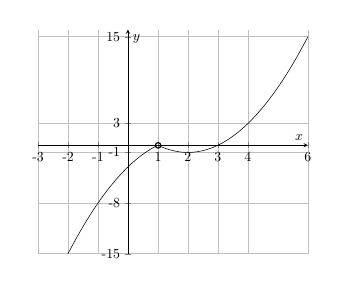
\begin{tikzpicture}[scale=0.5]
\begin{axis}[
    axis lines = middle,
    grid=major,
    legend pos={south west},
    xlabel = {$x$},
    %xlabel style={below right},
    ylabel = {$y$},
    ymin=-15,
    ymax=16,
    xmin=-3,
    xmax=6,
    xtick={-4,-2,-3,-1,1,2,3,4,6},
    xticklabels={-4,-2,-3,-1,1,2,3,4,6},
    ytick={-15, -8,-1,3,15},
    yticklabels={-15, -8,-1,3,15},
                  ]
	\addplot[domain=-4:1, samples=100, color=black] {-(x*x-4*x+3)};
    \addplot[domain=1:6, samples=100, color=black] {x*x-4*x+3};
    %\addplot[domain=2.01:6, samples=100, color=black] {2/(2-x)};
   % \addplot[domain=-3:3, samples=100, color=black] {-x};
     %\addlegendentry{$\text{Рис. 1}$};
\end{axis}
\draw (3.05,2.75) circle (2pt);
\end{tikzpicture}$$
По графику найдём $m\in(-1;0).$\\
65. Обе параболы пересекают ось $y$ в точке с положительной ординатой, значит $a>0,\ c>0.$ Но у одной из парабол ветви должны быть направлены вниз, значит такого быть не может.\\
66.  Обе параболы пересекают ось $y$ в точке с отрицательной ординатой, значит $a<0,\ c<0.$ Но у одной из парабол ветви должны быть направлены вверх, значит такого быть не может.\\
67. $y=-\cfrac{4|x+2|}{x^2+2x}=-\cfrac{4|x+2|}{x(x+2)}=\begin{cases} -\cfrac{4}{x},\ x>-2,\\ \cfrac{4}{x},\ x<-2.\end{cases}$
$$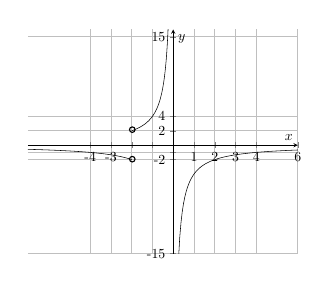
\begin{tikzpicture}[scale=0.5]
\begin{axis}[
    axis lines = middle,
    grid=major,
    legend pos={south west},
    xlabel = {$x$},
    %xlabel style={below right},
    ylabel = {$y$},
    ymin=-15,
    ymax=16,
    xmin=-7,
    xmax=6,
    xtick={-4,-3,-2,-1,1,2,3,4,6},
    xticklabels={-4,-3,$ $,$ $,1,2,3,4,6},
    ytick={-15, -2,-1,2,4,15},
    yticklabels={-15, -2,$ $,2,4,15},
                  ]
	\addplot[domain=-7:-2, samples=100, color=black] {(4/x)};
    \addplot[domain=-2:-0.01, samples=100, color=black] {-(4/x)};
    \addplot[domain=0.01:6, samples=100, color=black] {-(4/x)};
    %\addplot[domain=2.01:6, samples=100, color=black] {2/(2-x)};
   % \addplot[domain=-3:3, samples=100, color=black] {-x};
     %\addlegendentry{$\text{Рис. 1}$};
\end{axis}
\draw (2.65,3.15) circle (2pt);
\draw (2.65,2.4) circle (2pt);
\end{tikzpicture}$$
По графику определим $m\in(-\infty;-2]\cup(2;+\infty).$\\
68. $y=\cfrac{6|x-3|}{x^2-3x}=\cfrac{6|x-3|}{x(x-3)}=\begin{cases} \cfrac{6}{x},\ x>3,\\ -\cfrac{6}{x},\ x<3.\end{cases}$
$$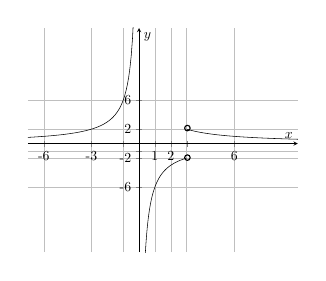
\begin{tikzpicture}[scale=0.5]
\begin{axis}[
    axis lines = middle,
    grid=major,
    legend pos={south west},
    xlabel = {$x$},
    %xlabel style={below right},
    ylabel = {$y$},
    ymin=-15,
    ymax=16,
    xmin=-7,
    xmax=10,
    xtick={-6,-3,-1,1,2,3,6},
    xticklabels={-6,-3,$ $,1,2,$ $,6},
    ytick={-1,-2,-6,2,6},
    yticklabels={$ $,-2,-6,2,6},
                  ]
	\addplot[domain=3:10, samples=100, color=black] {(6/x)};
    \addplot[domain=-8:-0.01, samples=100, color=black] {-(6/x)};
    \addplot[domain=0.01:3, samples=100, color=black] {-(6/x)};
    %\addplot[domain=2.01:6, samples=100, color=black] {2/(2-x)};
   % \addplot[domain=-3:3, samples=100, color=black] {-x};
     %\addlegendentry{$\text{Рис. 1}$};
\end{axis}
\draw (4.05,3.15) circle (2pt);
\draw (4.05,2.4) circle (2pt);
\end{tikzpicture}$$
По графику определим $m\in(-\infty;-2]\cup(2;+\infty).$\\
69. $y=\cfrac{2x^2-8x}{|x-2|-2}=\begin{cases}\cfrac{2x(x-4)}{x-4}=2x,\ x\geqslant2,\ x
eq4,\\ \cfrac{2x(x-4)}{-x}=8-2x,\ x<2,\ x
eq0.\end{cases}$
$$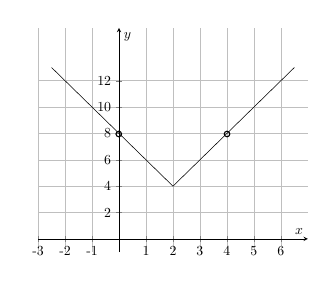
\begin{tikzpicture}[scale=0.5]
\begin{axis}[
    axis lines = middle,
    grid=major,
    legend pos={south west},
    xlabel = {$x$},
    %xlabel style={below right},
    ylabel = {$y$},
    ymin=-1,
    ymax=16,
    xmin=-3,
    xmax=7,
    xtick={-3,-2,-1,1,2,3,4,5,6},
    xticklabels={-3,-2,-1,1,2,3,4,5,6},
    ytick={2,4,6,8,10,12},
    yticklabels={2,4,6,8,10,12},
                  ]
	\addplot[domain=-2.5:2, samples=100, color=black] {2*(4-x)};
    \addplot[domain=2:6.5, samples=100, color=black] {(2*x)};
        %\addplot[domain=2.01:6, samples=100, color=black] {2/(2-x)};
   % \addplot[domain=-3:3, samples=100, color=black] {-x};
     %\addlegendentry{$\text{Рис. 1}$};
\end{axis}
\draw (2.05,3) circle (2pt);
\draw (4.8,3) circle (2pt);
\end{tikzpicture}$$
По графику найдём значение $y=4.$\\
70. $y=\cfrac{3x^2-6x}{|x-1|-1}=\begin{cases}\cfrac{3x(x-2)}{x-2}=3x,\ x\geqslant1,\ x
eq2,\\ \cfrac{3x(x-2)}{-x}=6-3x,\ x<1,\ x
eq0.\end{cases}$
$$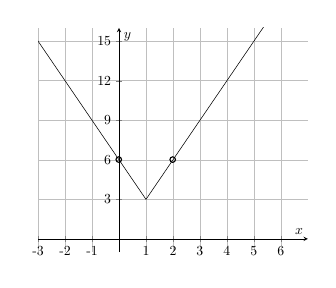
\begin{tikzpicture}[scale=0.5]
\begin{axis}[
    axis lines = middle,
    grid=major,
    legend pos={south west},
    xlabel = {$x$},
    %xlabel style={below right},
    ylabel = {$y$},
    ymin=-1,
    ymax=16,
    xmin=-3,
    xmax=7,
    xtick={-3,-2,-1,1,2,3,4,5,6},
    xticklabels={-3,-2,-1,1,2,3,4,5,6},
    ytick={3,6,9,12,15},
    yticklabels={3,6,9,12,15},
                  ]
	\addplot[domain=-3.5:1, samples=100, color=black] {3*(2-x)};
    \addplot[domain=1:5.5, samples=100, color=black] {(3*x)};
        %\addplot[domain=2.01:6, samples=100, color=black] {2/(2-x)};
   % \addplot[domain=-3:3, samples=100, color=black] {-x};
     %\addlegendentry{$\text{Рис. 1}$};
\end{axis}
\draw (2.05,2.35) circle (2pt);
\draw (3.42,2.35) circle (2pt);
\end{tikzpicture}$$
По графику найдём значение $y=3.$\\
71. У параболы $y=a(x-1)(x-4)=a(x^2-5x+4)=ax^2-5ax+4a$ вершина находится в точке $x_{\text{верш}}=-\cfrac{-5a}{2a}=2,5,$ а не 2. Значит, изображённая на рисунке парабола не может быть её графиком.\\
72. У параболы $y=a(x-2)(x-5)=a(x^2-7x+10)=ax^2-7ax+10a$ вершина находится в точке $x_{\text{верш}}=-\cfrac{-7a}{2a}=3,5,$ а не 3. Значит, изображённая на рисунке парабола не может быть её графиком.\\
73. Если $f(x)$ является нечётной функцией, то  $f(x)=\begin{cases}-\cfrac{2}{x^2},\ x<0,\\ \cfrac{2}{x^2},\ x>0.\end{cases}$
$$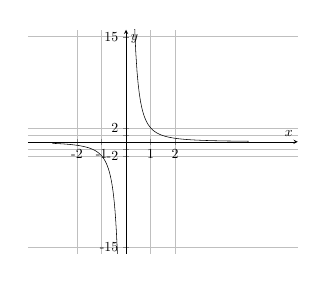
\begin{tikzpicture}[scale=0.5]
\begin{axis}[
    axis lines = middle,
    grid=major,
    legend pos={south west},
    xlabel = {$x$},
    %xlabel style={below right},
    ylabel = {$y$},
    ymin=-16,
    ymax=16,
    xmin=-4,
    xmax=7,
    xtick={-2,-1,1,2},
    xticklabels={-2,-1,1,2},
    ytick={-15,-2,-1,1,2,15},
    yticklabels={-15,-2,$ $,$ $,2,15},
                  ]
	\addplot[domain=-3:-0.1, samples=100, color=black] {-2/(x*x)};
    \addplot[domain=0.1:5, samples=100, color=black] {2/(x*x)};
        %\addplot[domain=2.01:6, samples=100, color=black] {2/(2-x)};
   % \addplot[domain=-3:3, samples=100, color=black] {-x};
     %\addlegendentry{$\text{Рис. 1}$};
\end{axis}
\end{tikzpicture}$$
74. $y=\cfrac{2x-3}{|x+2|}=\begin{cases}\cfrac{2x-3}{x+2},\ x>-2,\\ \cfrac{2x-3}{-x-2},\ x<-2.\end{cases}=
\begin{cases}2-\cfrac{7}{x+2},\ x>-2,\\ -2+\cfrac{7}{x+2},\ x<-2.\end{cases}$
$$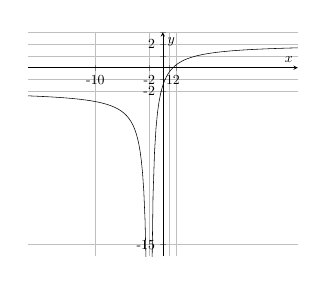
\begin{tikzpicture}[scale=0.5]
\begin{axis}[
    axis lines = middle,
    grid=major,
    legend pos={south west},
    xlabel = {$x$},
    %xlabel style={below right},
    ylabel = {$y$},
    ymin=-16,
    ymax=3,
    xmin=-20,
    xmax=20,
    xtick={-2,1,2,-10},
    xticklabels={-2,1,2,-10},
    ytick={-15,-2,-1,1,2,3},
    yticklabels={-15,-2,$ $,$ $,2,$ $},
                  ]
	\addplot[domain=-20:-2.1, samples=100, color=black] {(2*x-3)/abs(x+2)};
    \addplot[domain=-1.9:20, samples=100, color=black] {(2*x-3)/abs(x+2)};
        %\addplot[domain=2.01:6, samples=100, color=black] {2/(2-x)};
   % \addplot[domain=-3:3, samples=100, color=black] {-x};
     %\addlegendentry{$\text{Рис. 1}$};
\end{axis}
\end{tikzpicture}$$
75. У точки на оси ординат абсцисса равна нулю, то есть $\cfrac{k}{0-2}=0+1,\ k=-2.$\\
76. $y=\cfrac{x^3-x}{|x|}=\cfrac{x(x^2-1)}{|x|}=\begin{cases} x^2-1,\ x>0,\\ 1-x^2,\ x<0.\end{cases}$
$$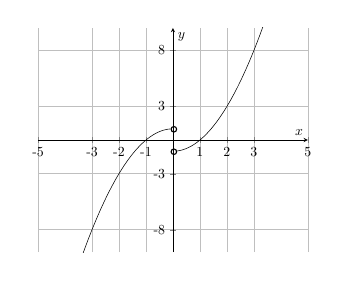
\begin{tikzpicture}[scale=0.5]
\begin{axis}[
    axis lines = middle,
    grid=major,
    legend pos={south west},
    xlabel = {$x$},
    %xlabel style={below right},
    ylabel = {$y$},
    ymin=-10,
    ymax=10,
    xmin=-5,
    xmax=5,
    xtick={-5,-3,-2,-1,1,2,3,5},
    xticklabels={-5,-3,-2,-1,1,2,3,5},
    ytick={-8,8,3,-3},
    yticklabels={-8,8,3,-3},
                  ]
	\addplot[domain=-5:-0.1, samples=100, color=black] {(x*x*x-x)/abs(x)};
    \addplot[domain=0.1:5, samples=100, color=black] {(x*x*x-x)/abs(x)};
        %\addplot[domain=2.01:6, samples=100, color=black] {2/(2-x)};
   % \addplot[domain=-3:3, samples=100, color=black] {-x};
     %\addlegendentry{$\text{Рис. 1}$};
\end{axis}
\draw (3.45,3.12) circle (2pt);
\draw (3.45,2.55) circle (2pt);
\end{tikzpicture}$$
77. $y=|x^2-4x|=\begin{cases} x^2-4x,\ x\leqslant0,\\ 4x-x^2,\ 0<x<4,\\ x^2-4x.\ x\geqslant4.\end{cases}$
$$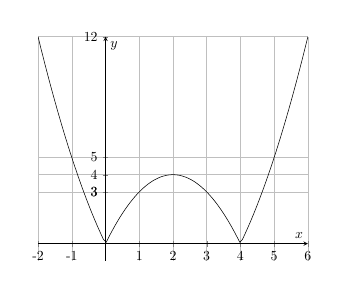
\begin{tikzpicture}[scale=0.5]
\begin{axis}[
    axis lines = middle,
    grid=major,
    legend pos={south west},
    xlabel = {$x$},
    %xlabel style={below right},
    ylabel = {$y$},
    ymin=-1,
    ymax=12,
    xmin=-2,
    xmax=6,
    xtick={-2,-1,1,2,3,4,5,6},
    xticklabels={-2,-1,1,2,3,4,5,6},
    ytick={5,3,12,3,4},
    yticklabels={5,3,12,3,4},
                  ]
	\addplot[domain=-2:6, samples=100, color=black] {abs(x*x-4*x)};
   % \addplot[domain=-3:3, samples=100, color=black] {-x};
     %\addlegendentry{$\text{Рис. 1}$};
\end{axis}
\end{tikzpicture}$$
 По графику найдём $a\in\{0\}\cup(4;+\infty).$\\
78. $f(x)=\cfrac{|x^2-3x|(x+1)}{x}=\cfrac{|x||x-3|(x+1)}{x}=\begin{cases} x^2-2x-3,\ x\geqslant3,\\ -x^2+2x+3,\ 0<x<3,\\ x^2-2x-3,\ x<0.\end{cases}$
$$\begin{tikzpicture}[scale=0.5]
\begin{axis}[
    axis lines = middle,
    grid=major,
    legend pos={south west},
    xlabel = {$x$},
    %xlabel style={below right},
    ylabel = {$y$},
    ymin=-4,
    ymax=13,
    xmin=-6,
    xmax=6,
    xtick={-5,-3,-2,-1,1,2,3,5},
    xticklabels={-5,-3,-2,-1,1,2,3,5},
    ytick={12,3,-3,4,5},
    yticklabels={12,3,-3,4,5},
                  ]
	\addplot[domain=-6:0, samples=100, color=black] {-abs(x-3)*(x+1)};
    \addplot[domain=0:6, samples=100, color=black] {abs(x-3)*(x+1)};
        %\addplot[domain=2.01:6, samples=100, color=black] {2/(2-x)};
   % \addplot[domain=-3:3, samples=100, color=black] {-x};
     %\addlegendentry{$\text{Рис. 1}$};
\end{axis}
\draw (3.45,2.35) circle (2pt);
\draw (3.45,0.35) circle (2pt);
%\draw (3.45,2.55) circle (2pt);
\end{tikzpicture}$$
79.  $f(x)=\cfrac{|x^2+2x|(x-1)}{x}=\cfrac{|x||x+2|(x-1)}{x}=\begin{cases} x^2+x-2,\ x>0,\\ -x^2-x+2,\ -2<x<0,\\ x^2+x-2,\ x\leqslant-2.\end{cases}$
$$\begin{tikzpicture}[scale=0.5]
\begin{axis}[
    axis lines = middle,
    grid=major,
    legend pos={south west},
    xlabel = {$x$},
    %xlabel style={below right},
    ylabel = {$y$},
    ymin=-4,
    ymax=11,
    xmin=-6,
    xmax=6,
    xtick={-5,-3,-2,-1,1,2,3,5},
    xticklabels={-5,-3,-2,-1,1,2,3,5},
    ytick={10,2,-2,4},
    yticklabels={10,2,-2,4},
                  ]
	\addplot[domain=-6:0, samples=100, color=black] {-abs(x+2)*(x-1)};
    \addplot[domain=0:6, samples=100, color=black] {abs(x+2)*(x-1)};
        %\addplot[domain=2.01:6, samples=100, color=black] {2/(2-x)};
   % \addplot[domain=-3:3, samples=100, color=black] {-x};
     %\addlegendentry{$\text{Рис. 1}$};
\end{axis}
\draw (3.45,2.25) circle (2pt);
\draw (3.45,0.75) circle (2pt);
%\draw (3.45,2.55) circle (2pt);
\end{tikzpicture}$$
80. $g(x)=\cfrac{2x+1}{2x^2+x}=\cfrac{2x+1}{x(2x+1)}=\cfrac{1}{x},\ x
eq-\cfrac{1}{2}.$
$$\begin{tikzpicture}[scale=0.5]
\begin{axis}[
    axis lines = middle,
    grid=major,
    legend pos={south west},
    xlabel = {$x$},
    %xlabel style={below right},
    ylabel = {$y$},
    ymin=-6,
    ymax=6,
    xmin=-2,
    xmax=2,
    xtick={-2, -2, -0.5, 1, 2},
    xticklabels={-2, -2, $-\frac{1}{2}$, 1, 2},
    ytick={-2,1},
    yticklabels={-2,1},
                  ]
	\addplot[domain=-2:-0.1, samples=100, color=black] {1/x};
    \addplot[domain=0.1:2, samples=100, color=black] {1/x};
        %\addplot[domain=2.01:6, samples=100, color=black] {2/(2-x)};
   % \addplot[domain=-3:3, samples=100, color=black] {-x};
     %\addlegendentry{$\text{Рис. 1}$};
\end{axis}
\draw (2.57,1.86) circle (2pt);
%\draw (3.45,0.75) circle (2pt);
%\draw (3.45,2.55) circle (2pt);
\end{tikzpicture}$$
а) Прямая $y=kx$ имеет с графиком $g(x)$ одну общую точку, если проходит через точку $\left(-\cfrac{1}{2};-2
ight),$ то есть если $-\cfrac{1}{2}k=-2,\ k=4.$\\
б) Для нахождения общих точек графика и прямой, составим уравнение $\cfrac{1}{x}=bx+2,\ bx^2+2x-1=0,$ при этом $x
eq-\cfrac{1}{2}.$ Это уравнение имеет один корень либо при $b=0$ $\left(\text{тогда }x=\cfrac{1}{2}
ight),$ либо при $\cfrac{D}{4}=1+b=0,\ b=-1\ \left(\text{тогда }x=1
ight),$ либо если одним из корней является $x=-\cfrac{1}{2},$ то есть $b\cdot\cfrac{1}{4}-1-1=0,\ b=8.$\\
81. $g(x)=\cfrac{x-2}{2x-x^2}=\cfrac{x-2}{x(2-x)}=-\cfrac{1}{x},\ x
eq2.$
$$\begin{tikzpicture}[scale=0.5]
\begin{axis}[
    axis lines = middle,
    grid=major,
    legend pos={south west},
    xlabel = {$x$},
    %xlabel style={below right},
    ylabel = {$y$},
    ymin=-6,
    ymax=6,
    xmin=-3,
    xmax=3,
    xtick={-2, -2,  1, 2},
    xticklabels={-2, -2, 1, $ $},
    ytick={-2,-0.5, 1},
    yticklabels={-2,$-\frac{1}{2}$, 1},
                  ]
	\addplot[domain=-3:-0.1, samples=100, color=black] {-1/x};
    \addplot[domain=0.1:3, samples=100, color=black] {-1/x};
        %\addplot[domain=2.01:6, samples=100, color=black] {2/(2-x)};
   % \addplot[domain=-3:3, samples=100, color=black] {-x};
     %\addlegendentry{$\text{Рис. 1}$};
\end{axis}
\draw (5.71,2.59) circle (2pt);
%\draw (3.45,0.75) circle (2pt);
%\draw (3.45,2.55) circle (2pt);
\end{tikzpicture}$$
а) Прямая $y=kx$ имеет с графиком $g(x)$ одну общую точку, если проходит через точку $\left(2;-\cfrac{1}{2}
ight),$ то есть если $2k=-\cfrac{1}{2},\ k=-\cfrac{1}{4}.$\\
б) Для нахождения общих точек графика и прямой, составим уравнение $-\cfrac{1}{x}=bx+2,\ bx^2+2x+1=0,$ при этом $x
eq2.$ Это уравнение имеет один корень либо при $b=0$ $\left(\text{тогда }x=-\cfrac{1}{2}
ight),$ либо при $\cfrac{D}{4}=1-b=0,\ b=1\ \left(\text{тогда }x=-1
ight),$ либо если одним из корней является $x=2,$ то есть $b\cdot4+4+1=0,\ b=-\cfrac{5}{4}.$\\
82. $f(x)=\cfrac{2-|x+3|}{x}=\begin{cases} \cfrac{2+x+3}{x},\ x\leqslant-3,\\
\cfrac{2-x-3}{x},\ x>-3.\end{cases}=\begin{cases} 1+\cfrac{5}{x},\ x\leqslant-3,\\
-1-\cfrac{1}{x},\ x>-3.\end{cases}$\\
а) $$\begin{tikzpicture}[scale=0.5]
\begin{axis}[
    axis lines = middle,
    grid=major,
    legend pos={south west},
    xlabel = {$x$},
    %xlabel style={below right},
    ylabel = {$y$},
    ymin=-10,
    ymax=10,
    xmin=-10,
    xmax=6,
    xtick={-5, -3,  1, 2},
    xticklabels={-5, -3, 1, $ $},
    ytick={-2,-0.66, 1},
    yticklabels={-2,$-\frac{2}{3}$, 1},
                  ]
	\addplot[domain=-10:-3, samples=100, color=black] {1+5/x};
    \addplot[domain=-2.99:6, samples=100, color=black] {-1-1/x};
        %\addplot[domain=2.01:6, samples=100, color=black] {2/(2-x)};
   % \addplot[domain=-3:3, samples=100, color=black] {-x};
     %\addlegendentry{$\text{Рис. 1}$};
\end{axis}
%\draw (5.71,2.59) circle (2pt);
%\draw (3.45,0.75) circle (2pt);
%\draw (3.45,2.55) circle (2pt);
\end{tikzpicture}$$
б) При $x<0$ график функции находится выше уровня $y=-\cfrac{3}{2}.$ Если $-1-\cfrac{1}{x}=-\cfrac{3}{2},$ то $\cfrac{1}{x}=\cfrac{1}{2},\ x=2.$ Значит, $f(x)\geqslant -\cfrac{3}{2}$ при $x\in(-\infty;0)\cup[2;+\infty).$\\
в) Горизонтальными асимптотами являются $y=-1$ и $y=1,$ исходя из этого найдём количество решений: при $a\in\left[-1;-\cfrac{2}{3}
ight):0,$ при $a\in(-\infty;-1)\cup\left\{-\cfrac{2}{3}
ight\}\cup[1;+\infty):1,$ при $a\in\left(-\cfrac{2}{3};1
ight):2.$\\
83. $f(x)=\cfrac{1-|x-2|}{x}=\begin{cases} \cfrac{1+x-2}{x},\ x\leqslant2,\\
\cfrac{1-x+2}{x},\ x>2.\end{cases}=\begin{cases} 1-\cfrac{1}{x},\ x\leqslant2,\\
-1+\cfrac{3}{x},\ x>2.\end{cases}$\\
а) $$\begin{tikzpicture}[scale=0.5]
\begin{axis}[
    axis lines = middle,
    grid=major,
    legend pos={south west},
    xlabel = {$x$},
    %xlabel style={below right},
    ylabel = {$y$},
    ymin=-10,
    ymax=10,
    xmin=-10,
    xmax=6,
    xtick={-5, -2,  1, 2},
    xticklabels={-5, -2, 1, 2},
    ytick={-1, 0.5, 1, 1.5},
    yticklabels={-1, $\frac{1}{2}$, $ $, $  $},
                  ]
	\addplot[domain=-10:2, samples=100, color=black] {1-1/x};
    \addplot[domain=2.01:10, samples=100, color=black] {-1+3/x};
        %\addplot[domain=2.01:6, samples=100, color=black] {2/(2-x)};
   % \addplot[domain=-3:3, samples=100, color=black] {-x};
     %\addlegendentry{$\text{Рис. 1}$};
\end{axis}
%\draw (5.71,2.59) circle (2pt);
%\draw (3.45,0.75) circle (2pt);
%\draw (3.45,2.55) circle (2pt);
\end{tikzpicture}$$
б) При $x>0$ график функции находится ниже уровня $y=\cfrac{3}{2}.$ Если $1-\cfrac{1}{x}=\cfrac{3}{2},$ то $\cfrac{1}{x}=-\cfrac{1}{2},\ x=-2.$ Значит, $f(x)\leqslant \cfrac{3}{2}$ при $x\in(-\infty;-2]\cup(0;+\infty).$\\
в) Горизонтальными асимптотами являются $y=-1$ и $y=1,$ исходя из этого найдём количество решений: при $a\in\left(\cfrac{1}{2};1
ight]:0,$ при $a\in(-\infty;-1]\cup\left\{\cfrac{1}{2}
ight\}\cup(1;+\infty):1,$ при $a\in\left(-1;\cfrac{1}{2}
ight):2.$\\
84. $f(x)=\begin{cases} \sqrt{1-x},\ \text{ если } x\leqslant0,\\
x^2-|2x+1|,\ \text{ если } x>0.\end{cases}=\begin{cases} \sqrt{1-x},\ \text{ если } x\leqslant0,\\
x^2-2x-1,\ \text{ если } x>0.\end{cases}$
$$\begin{tikzpicture}[scale=0.5]
\begin{axis}[
    axis lines = middle,
    grid=major,
    legend pos={south west},
    xlabel = {$x$},
    %xlabel style={below right},
    ylabel = {$y$},
    ymin=-5,
    ymax=10,
    xmin=-10,
    xmax=6,
    xtick={-8, -3, 1, 4},
    xticklabels={-8, -3, 1, 4},
    ytick={-2,2, 3, 7},
    yticklabels={-2,2, 3, 7},
                  ]
	\addplot[domain=-10:0, samples=100, color=black] {sqrt(1-x)};
    \addplot[domain=0.01:10, samples=100, color=black] {x*x-2*x-1};
        %\addplot[domain=2.01:6, samples=100, color=black] {2/(2-x)};
   % \addplot[domain=-3:3, samples=100, color=black] {-x};
     %\addlegendentry{$\text{Рис. 1}$};
\end{axis}
\draw (4.3,1.5) circle (2pt);
%\draw (3.45,0.75) circle (2pt);
%\draw (3.45,2.55) circle (2pt);
\end{tikzpicture}$$
85. $f(x)=\begin{cases} 2, \text{ если } x>1,\\ -1, \text{ если } x<1,\\ 1, \text{ если } x=1.\end{cases}$
Так как $\sqrt{x-2}=1$ при $x=3,\ f(\sqrt{x-2})=1$ при $x=3.$ Так как $\sqrt{x-2}>1$ при $x>3,\ f(\sqrt{x-2})=2$ при $x>3.$ При $x\in[2;3)$ имеем неравенство
$\sqrt{x-2}<1,$ значит $f(\sqrt{x-2})=-1$ при $x\in[2;3).$ Исходя их этого, построим график.
\begin{figure}[ht!]
\center{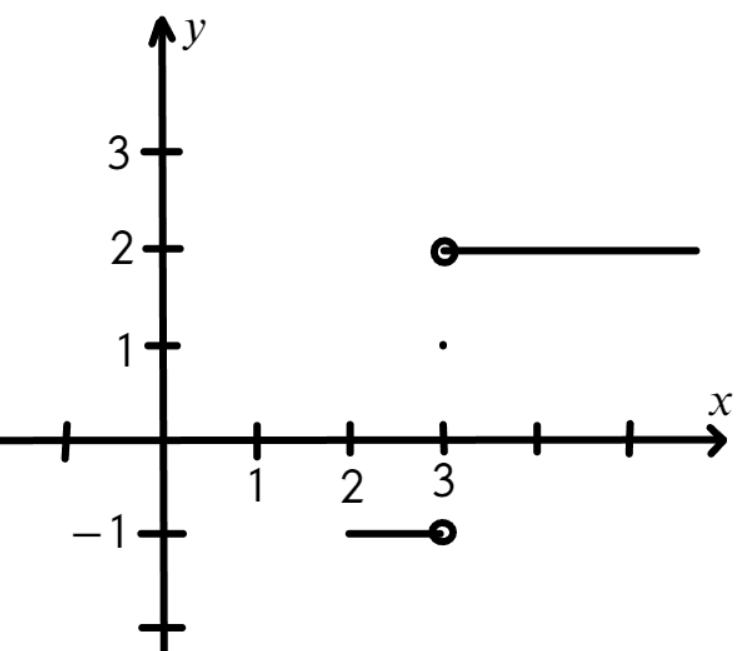
\includegraphics[scale=0.35]{gr9-85.png}}
\end{figure}\\
86. $f(x)=\cfrac{1-|x-2|}{x}=\begin{cases} \cfrac{1+x-2}{x},\ x\leqslant 2,\\ \cfrac{1-x+2}{x},\ x > 2.\end{cases}=\begin{cases} 1-\cfrac{1}{x},\ x\leqslant 2,\\ \cfrac{3}{x}-1,\ x > 2.\end{cases}$
$$\begin{tikzpicture}[scale=0.5]
\begin{axis}[
    axis lines = middle,
    grid=major,
    legend pos={south west},
    xlabel = {$x$},
    %xlabel style={below right},
    ylabel = {$y$},
    ymin=-15,
    ymax=16,
    xmin=-7,
    xmax=6,
    xtick={-4,-3,-1,1,2,3,4,6},
    xticklabels={-4,-3,-1,1,2,3,4,6},
    ytick={-15,-1,0.5,2,15},
    yticklabels={-15, $ $,0.5,2,15},
                  ]
    \addplot[domain=-6:-0.01, samples=100, color=black] {1-(1/x)};
	\addplot[domain=0.01:2, samples=100, color=black] {1-(1/x)};
    \addplot[domain=2:6, samples=100, color=black] {-1+(3/x)};
    %\addplot[domain=2.01:6, samples=100, color=black] {2/(2-x)};
   % \addplot[domain=-3:3, samples=100, color=black] {-x};
     %\addlegendentry{$\text{Рис. 1}$};
\end{axis}
\end{tikzpicture}$$
По графику определим ответ $x\in(-\infty;-1]\cup(0;+\infty).$\\
87. $f(x)=\cfrac{2-|x+3|}{x}=\begin{cases} \cfrac{2+x+3}{x},\ x\leqslant -3,\\ \cfrac{2-x-3}{x},\ x > -3.\end{cases}=\begin{cases} 1+\cfrac{5}{x},\ x\leqslant -3,\\ -\cfrac{1}{x}-1,\ x > -3.\end{cases}$
$$\begin{tikzpicture}[scale=0.5]
\begin{axis}[
    axis lines = middle,
    grid=major,
    legend pos={south west},
    xlabel = {$x$},
    %xlabel style={below right},
    ylabel = {$y$},
    ymin=-15,
    ymax=16,
    xmin=-7,
    xmax=6,
    xtick={-5, -3,1,3,6},
    xticklabels={-5,-3,1,3,6},
    ytick={-15,-2,-1, -0.666,1, 15},
    yticklabels={-15, -2,$ $,$ $,1, 15},
                  ]
    \addplot[domain=-10:-3, samples=100, color=black] {1+(5/x)};
	\addplot[domain=-3:-0.01, samples=100, color=black] {-1-(1/x)};
    \addplot[domain=0.01:6, samples=100, color=black] {-1-(1/x)};
    %\addplot[domain=2.01:6, samples=100, color=black] {2/(2-x)};
   % \addplot[domain=-3:3, samples=100, color=black] {-x};
     %\addlegendentry{$\text{Рис. 1}$};
\end{axis}
\end{tikzpicture}$$
По графику определим ответ $x\in(-\infty;-0)\cup[1;+\infty).$\\
88. Для построения графика функции $f(x)=|x^2-6x+5|$ сначала построим параболу $y=x^2-6x+5=(x-1)(x-5).$ После этого отразим её отрицательную часть при $x\in(1;5)$ наверх относительно оси абсцисс. Её вершина $(3;-4)$ отразится в точку $(3;4).$ График функции $g(x)=k(x-7)+4$ при любом значении $k$ проходит через точку $(7;4).$  С графиком функции $f(x)$ он может иметь три общие точки только в двух случаях: если параллелен оси абсцисс, тогда $k=0,$ или если проходит через точку $(1;0),$ в этом случае $0=k\cdot(-6)+4,\ k=\cfrac{2}{3}.$
$$\begin{tikzpicture}[scale=0.5]
\begin{axis}[
    axis lines = middle,
    grid=major,
    legend pos={south west},
    xlabel = {$x$},
    %xlabel style={below right},
    ylabel = {$y$},
    ymin=-1,
    ymax=16,
    xmin=-2,
    xmax=10,
    xtick={-2,-1,1,2,3,4,5,6,7},
    xticklabels={-2,-1,1,2,3,4,5,6,7},
    ytick={2,4,5,12},
    yticklabels={2,4,5,12},
                  ]
	\addplot[domain=-4:10, samples=100, color=black] {abs(x*x-6*x+5)};
        %\addplot[domain=2.01:6, samples=100, color=black] {2/(2-x)};
   % \addplot[domain=-3:3, samples=100, color=black] {-x};
     %\addlegendentry{$\text{Рис. 1}$};
\end{axis}
\end{tikzpicture}$$
89. Для построения графика функции $f(x)=|x^2+2x-3|$ сначала построим параболу $y=x^2+2x-3=(x-1)(x+3).$ После этого отразим её отрицательную часть при $x\in(-3;1)$ наверх относительно оси абсцисс. Её вершина $(-1;-4)$ отразится в точку $(1;4).$ График функции $g(x)=k(x+5)+4$ при любом значении $k$ проходит через точку $(-5;4).$  С графиком функции $f(x)$ он может иметь три общие точки только в двух случаях: если параллелен оси абсцисс, тогда $k=0,$ или если проходит через точку $(1;0),$ в этом случае $0=k\cdot6+4,\ k=-\cfrac{2}{3}.$
$$\begin{tikzpicture}[scale=0.5]
\begin{axis}[
    axis lines = middle,
    grid=major,
    legend pos={south west},
    xlabel = {$x$},
    %xlabel style={below right},
    ylabel = {$y$},
    ymin=-1,
    ymax=16,
    xmin=-8,
    xmax=5,
    xtick={-5,-1,1,2,3,4},
    xticklabels={-5,-1,1,2,3,4},
    ytick={2,4,5,12},
    yticklabels={2,4,5,12},
                  ]
	\addplot[domain=-6:5, samples=100, color=black] {abs(x*x+2*x-3)};
        %\addplot[domain=2.01:6, samples=100, color=black] {2/(2-x)};
   % \addplot[domain=-3:3, samples=100, color=black] {-x};
     %\addlegendentry{$\text{Рис. 1}$};
\end{axis}
\end{tikzpicture}$$
90. а) $f(x)=x^2-|2x-1|=\begin{cases} x^2+2x-1,\ x\leqslant\cfrac{1}{2},\\ x^2-2x+1,\ x>\cfrac{1}{2}.\end{cases}$
$$\begin{tikzpicture}[scale=0.5]
\begin{axis}[
    axis lines = middle,
    grid=major,
    legend pos={south west},
    xlabel = {$x$},
    %xlabel style={below right},
    ylabel = {$y$},
    ymin=-3,
    ymax=2,
    xmin=-3,
    xmax=3,
    xtick={-2,-1,0.5, 1,2},
    xticklabels={-2, -1,0.5, 1,2},
    ytick={-2,-1,0.25,1},
    yticklabels={-2,-1,0.25,1},
                  ]
	\addplot[domain=-4:0.5, samples=100, color=black] {(x*x+2*x-1)};
\addplot[domain=0.5:3, samples=100, color=black] {(x*x-2*x+1)};
        %\addplot[domain=2.01:6, samples=100, color=black] {2/(2-x)};
   % \addplot[domain=-3:3, samples=100, color=black] {-x};
     %\addlegendentry{$\text{Рис. 1}$};
\end{axis}
\end{tikzpicture}$$
б) По графику определим количество пересечений функции $f(x)=x^2-|2x-1|$ с горизонтальной прямой $y=a,$ два пересечения будут при $a\in(-2;0)\cup\left(\cfrac{1}{4};+\infty
ight).$\\
91. Так как у параболы $f$ ветви направлены вверх, а у $g$ --- вниз, имеем соотношения $a_1>0>a_2.$ Так как значения $f$ и $g$ при $x=0$ совпадают, имеем равенство $c_1=c_2.$ Так как параболы касаются, уравнение $f(x)=g(x)$ имеет ровно одно решение $x=0.$ Но если $a_1x^2+b_1x+c_1=a_2x^2+b_2x+c_2,$ то с учётом равенства $c_1=c_2$ и того, что $a_1-a_2
eq0,$ получим второй корень $x=\cfrac{b_2-b_1}{a_1-a_2}.$ Так как второго корня быть не может, он совпадает с первым $x=0,$ а значит $b_1=b_2.$\\
92. $f(x)=\cfrac{x^2+x}{x}\cdot\sqrt{x^2-6x+9}=\cfrac{x(x+1)}{x}\cdot\sqrt{(x-3)^2}=\begin{cases}(x+1)|x-3|,\\ x
eq0.\end{cases}=$\\$
\begin{cases}x^2-2x-3,\ x\geqslant3,\\ -x^2+2x+3,\ x\in(-\infty;0)\cup(0;3).\end{cases}$
$$\begin{tikzpicture}[scale=0.5]
\begin{axis}[
    axis lines = middle,
    grid=major,
    legend pos={south west},
    xlabel = {$x$},
    %xlabel style={below right},
    ylabel = {$y$},
    ymin=-45,
    ymax=22,
    xmin=-6,
    xmax=6,
    xtick={-5,-3,-1, 1,3,5},
    xticklabels={-5,-3,-1, 1,3,5},
    ytick={-32,-12,3,12},
    yticklabels={-32,-12,3,12},
                  ]
	\addplot[domain=3:6, samples=100, color=black] {(x*x-2*x-3)};
\addplot[domain=-6:3, samples=100, color=black] {(-x*x+2*x+3)};
        %\addplot[domain=2.01:6, samples=100, color=black] {2/(2-x)};
   % \addplot[domain=-3:3, samples=100, color=black] {-x};
     %\addlegendentry{$\text{Рис. 1}$};
\end{axis}
\draw (3.42,4.08) circle (2pt);
\end{tikzpicture}$$
93. $f(x)=\cfrac{x^2+x-6}{2-x}\cdot\sqrt{x^2-2x+1}=\cfrac{(x-2)(x+3)}{2-x}\cdot\sqrt{(x-1)^2}=\begin{cases}-(x+3)|x-1|,\\ x
eq2.\end{cases}=$\\$
\begin{cases}-x^2-2x+3,\ x\in[1;2)\cup(2;+\infty),\\ x^2+2x-3,\ x<1.\end{cases}$
$$\begin{tikzpicture}[scale=0.5]
\begin{axis}[
    axis lines = middle,
    grid=major,
    legend pos={south west},
    xlabel = {$x$},
    %xlabel style={below right},
    ylabel = {$y$},
    ymin=-45,
    ymax=22,
    xmin=-6,
    xmax=6,
    xtick={-5,-3, 1,2, 5},
    xticklabels={-5,-3, 1,2, 5},
    ytick={-32,-5,12},
    yticklabels={-32,-5,12},
                  ]
	\addplot[domain=1:6, samples=100, color=black] {(-x*x-2*x+3)};
\addplot[domain=-6:1, samples=100, color=black] {(x*x+2*x-3)};
        %\addplot[domain=2.01:6, samples=100, color=black] {2/(2-x)};
   % \addplot[domain=-3:3, samples=100, color=black] {-x};
     %\addlegendentry{$\text{Рис. 1}$};
\end{axis}
\draw (4.57,3.37) circle (2pt);
\end{tikzpicture}$$
94. Единственное решение имеет уравнение $x^2+p=-4x-5,\ x^2+4x+(p+5),$ значит $D=16-4(p+5)=0,\ p+5=4, p=-1.$ Тогда $x^2+4x+4=0,\ (x+2)^2=0,\ x=-2,\ y=4-1=3,$ то есть точка их пересечния имеет координаты $(-2;3).$
$$\begin{tikzpicture}[scale=0.5]
\begin{axis}[
    axis lines = middle,
    grid=major,
    legend pos={south west},
    xlabel = {$x$},
    %xlabel style={below right},
    ylabel = {$y$},
    ymin=-26,
    ymax=24,
    xmin=-5,
    xmax=5,
    xtick={-5,-4,-2, 1,2, 3, 5},
    xticklabels={-5,-4,-2, 1,2, 3, 5},
    ytick={-25,-17,-4, 3, 8, 15, 24},
    yticklabels={-25,-17,-4, 3, 8, 15, 24},
                  ]
\addplot[domain=-5:5, samples=100, color=black] {(x*x-1)};
\addplot[domain=-5:5, samples=100, color=black] {(-4*x-5)};
        %\addplot[domain=2.01:6, samples=100, color=black] {2/(2-x)};
   % \addplot[domain=-3:3, samples=100, color=black] {-x};
     %\addlegendentry{$\text{Рис. 1}$};
\end{axis}

\end{tikzpicture}$$
95. а) $|2x-y|=x\Leftrightarrow \begin{cases}\left[\begin{array}{l}2x-y=x,\\2x-y=-x.\end{array}
ight.\\x\geqslant0.\end{cases}
\Leftrightarrow \begin{cases}\left[\begin{array}{l}y=x,\\ y=3x.\end{array}
ight.\\x\geqslant0.\end{cases}$
$$\begin{tikzpicture}[scale=0.5]
\begin{axis}[
    axis lines = middle,
    grid=major,
    legend pos={south west},
    xlabel = {$x$},
    %xlabel style={below right},
    ylabel = {$y$},
    ymin=-1,
    ymax=15,
    xmin=-1,
    xmax=5,
    xtick={ 1,2, 3,4, 5},
    xticklabels={1,2, 3,4, 5},
    ytick={1,2, 3, 5,9,12,15},
    yticklabels={1,2, 3, 5,9,12,15},
                  ]
\addplot[domain=0:5, samples=100, color=black] {x};
\addplot[domain=0:5, samples=100, color=black] {3*x};
        %\addplot[domain=2.01:6, samples=100, color=black] {2/(2-x)};
   % \addplot[domain=-3:3, samples=100, color=black] {-x};
     %\addlegendentry{$\text{Рис. 1}$};
\end{axis}

\end{tikzpicture}$$
б) $|2x-y|<x\Leftrightarrow \begin{cases}2x-y<x,\\ 2x-y>-x.\end{cases}
\Leftrightarrow \begin{cases}y>x,\\ y<3x.\end{cases}$
$$\begin{tikzpicture}[scale=0.2]
\tikzset {line01/.style={line width =0.5pt}}
\tikzset{line02/.style={line width =1pt}}
\tikzset{line03/.style={dashed,line width =0.5pt}}
%\filldraw [black] (0,0) circle (1pt);
\draw [->] (-1,0) -- (6,0);
\draw [->] (0,-1) -- (0,16);
\draw[line01] (1,1.05) -- (1,2.95);
\draw[line01] (2,2.05) -- (2,5.95);
\draw[line01] (3,3.05) -- (3,8.95);
\draw[line01] (4,4.05) -- (4,11.95);
\draw[line01] (5,5.05) -- (5,14.95);
\draw[line03] (0,0) -- (6,6);
%\draw[line01] (-2,-7) -- (-2,7);
\draw[line03] (0,0) -- (5,15);
%\draw[line03] (0,2) -- (1,2);
%\draw[line03] (0,-2) -- (1,-2);
\draw (6.2,0.7) node {\scriptsize $x$};
%\draw (-1.2,-2) node {\scriptsize $-2$};
%\draw (-0.7,2) node {\scriptsize $2$};
\draw (-0.7,6) node {\scriptsize $6$};
\draw (-0.7,3) node {\scriptsize $3$};
\draw (-0.7,9) node {\scriptsize $9$};
\draw (-0.8,12) node {\scriptsize $12$};
\draw (-0.8,15) node {\scriptsize $15$};

\draw (2,-0.7) node {\scriptsize $2$};
\draw (1,-0.7) node {\scriptsize $1$};
\draw (3,-0.7) node {\scriptsize $3$};
\draw (4,-0.7) node {\scriptsize $4$};
\draw (5,-0.7) node {\scriptsize $5$};
%\draw (0.7,-1) node {\tiny $-1$};

%\draw (-2.8,-0.9) node {\tiny $-2$};
\draw (0.7,15.2) node {\scriptsize $y$};
%\draw (1,2) circle (8pt);
%\draw (-2,-3) circle (8pt);
\end{tikzpicture}$$
96. а) $f(x)=\begin{cases} \cfrac{3x-1}{x+1},\ x
eq-1\\3+2,\ x=-1 \end{cases}=\begin{cases} 3-\cfrac{4}{x+1},\ x
eq-1\\5,\ x=-1 \end{cases}.$
$$\begin{tikzpicture}[scale=1]
\tikzset{line03/.style={dashed,line width =0.9pt}}
\begin{axis}[
    axis lines = middle,
    grid=major,
    legend pos={south west},
    xlabel = {$x$},
    %xlabel style={below right},
    ylabel = {$y$},
    ymin=-10,
    ymax=10,
    xmin=-10,
    xmax=10,
    xtick={-5, -3, -1, 1, 3},
    xticklabels={-5, -3, $\text{                     -1}$, 1, 3},
    ytick={4, 5, 1, 2},
    yticklabels={$\text{4          }$,$\text{5           }$, $\text{1          }$, $\text{2            }$},        ]

	\addplot[domain=-0.9:10, samples=100, color=black] {3-4/(x+1)};
	\addplot[domain=-10:-1.1, samples=100, color=black] {3-4/(x+1)};

\end{axis}
\filldraw [black] (3.11,4.25) circle (1.5pt);
\draw[line03] (3.11,0) -- (3.11,6);
\draw[line03] (0,3.7) -- (6.5,3.7);
%\draw (3,5.7) node {\scriptsize $y$};
%\draw (7,2.5) node {\scriptsize $x$};
\end{tikzpicture}$$
б) Горизонтальная прямая $y=a-1$ не пересекается с графиком данной функции только в том случае, если является его асимптотой, то есть $a-1=3,\ a=4.$\\
в) Прямая $y=ax+1$ имеет с графиком три общие точки, только если она пересекает гиперболу 2 раза (тогда $a<0$) и проходит через изолированную точку $(-1;a+2).$ Тогда $-a+1=a+2,\ 2a=-1,\ a=-\cfrac{1}{2}.$\\
97. а) $f(x)=\begin{cases} \cfrac{3x+1}{x-1},\ x
eq1\\3+1,\ x=1 \end{cases}=\begin{cases} 3+\cfrac{4}{x-1},\ x
eq1\\ 4,\ x=1 \end{cases}.$
$$\begin{tikzpicture}[scale=1]
\tikzset{line03/.style={dashed,line width =0.9pt}}
\begin{axis}[
    axis lines = middle,
    grid=major,
    legend pos={south west},
    xlabel = {$x$},
    %xlabel style={below right},
    ylabel = {$y$},
    ymin=-10,
    ymax=10,
    xmin=-10,
    xmax=10,
    xtick={ -3, -1, 1, 2, 3, 5},
    xticklabels={ -3, -1, $\text{1     }$, 2, 3, 5},
    ytick={2, 1, 7, 5, 4},
    yticklabels={$\text{2}$,$\text{1}$, $\text{7}$, $\text{5}$, $\text{4}$},        ]

	\addplot[domain=1.1:10, samples=100, color=black] {3+4/(x-1)};
	\addplot[domain=-10:0.9, samples=100, color=black] {3+4/(x-1)};

\end{axis}
\filldraw [black] (3.8,3.97) circle (1.5pt);
\draw[line03] (3.8,0) -- (3.8,6);
\draw[line03] (0,3.7) -- (6.5,3.7);
%\draw (3,5.7) node {\scriptsize $y$};
%\draw (7,2.5) node {\scriptsize $x$};
\end{tikzpicture}$$
б) Горизонтальная прямая $y=a+1$ не пересекается с графиком данной функции только в том случае, если является его асимптотой, то есть $a+1=3,\ a=2.$\\
в) Прямая $y=ax+2$ имеет с графиком три общие точки, только если она пересекает гиперболу 2 раза (тогда $a>0$) и проходит через изолированную точку $(1;3-a).$ Тогда $a+2=3-a,\ 2a=1,\ a=\cfrac{1}{2}.$\\
98. а) $f(x)=\begin{cases} 4-|x+1|,\ x<2\\ x^2-6x+4,\ x\geqslant 2\end{cases}$
$$\begin{tikzpicture}[scale=1]
\tikzset{line03/.style={dashed,line width =0.9pt}}
\begin{axis}[
    axis lines = middle,
    grid=major,
    legend pos={south west},
    xlabel = {$x$},
    %xlabel style={below right},
    ylabel = {$y$},
    ymin=-10,
    ymax=10,
    xmin=-10,
    xmax=10,
    xtick={-5, -3, -1, 1, 2, 3, 5.236},
    xticklabels={-5, -3, -1, 1, 2, 3, \tiny{     $3+\sqrt{5}$}},
    ytick={4, 2, -4, 1, -5},
    yticklabels={$\text{4                    }$, 2, -4, 1, -5},        ]

	\addplot[domain=2:10, samples=100, color=black] {x*x-6*x+4};
	\addplot[domain=-10:1.95, samples=100, color=black] {4-abs(x+1)};

\end{axis}
\draw  (4.1,3.15) circle (1.5pt);
%\draw[line03] (3.11,0) -- (3.11,6);
%\draw[line03] (0,3.7) -- (6.5,3.7);
%\draw (3,5.7) node {\scriptsize $y$};
%\draw (7,2.5) node {\scriptsize $x$};
\end{tikzpicture}$$
б) По графику определим, что горизонатльная прямая $y=2a$ пересекает график функции $f(x)$ дважды в следующих случаях:
$2a=-5,\ 2a=4$ или $2a\in(-4;1],$ таким образом $a\in\left(-2;\cfrac{1}{2}
ight]\cup\left\{-\cfrac{5}{2};2
ight\}.$\\
99. а) $f(x)=\begin{cases} |x-3|-4,\ x>1\\ -x^2-3x+4,\ x\leqslant 1\end{cases}$
$$\begin{tikzpicture}[scale=1]
\tikzset{line03/.style={dashed,line width =0.9pt}}
\begin{axis}[
    axis lines = middle,
    grid=major,
    legend pos={south west},
    xlabel = {$x$},
    %xlabel style={below right},
    ylabel = {$y$},
    ymin=-10,
    ymax=10,
    xmin=-10,
    xmax=10,
    xtick={-4, -1.5, 1, 3, 5},
    xticklabels={-4, \tiny{$-\frac{3}{2}$}, 1, 3, 5},
    ytick={6.25, 4, -4, 1, -2},
    yticklabels={\tiny{$\frac{25}{4}$}, 4, -4, 1, \tiny{-2}},        ]

	\addplot[domain=1.05:10, samples=100, color=black] {abs(x-3)-4};
	\addplot[domain=-10:1, samples=100, color=black] {-x*x-3*x+4};

\end{axis}
\draw  (3.8,2.27) circle (1.5pt);
%\draw[line03] (3.11,0) -- (3.11,6);
%\draw[line03] (0,3.7) -- (6.5,3.7);
%\draw (3,5.7) node {\scriptsize $y$};
%\draw (7,2.5) node {\scriptsize $x$};
\end{tikzpicture}$$
б) По графику определим, что горизонатльная прямая $y=\cfrac{a}{2}$ пересекает график функции $f(x)$ дважды в следующих случаях:
$\cfrac{a}{2}=-4,\ \cfrac{a}{2}=\cfrac{25}{4}$ или $\cfrac{a}{2}\in[-2;0),$ таким образом $a\in\left[-4;0
ight)\cup\left\{-8;\cfrac{25}{2}
ight\}.$\\
100. $$\begin{tikzpicture}[scale=0.5]
\begin{axis}[
    axis lines = middle,
    grid=major,
    legend pos={south west},
    xlabel = {$x$},
    %xlabel style={below right},
    ylabel = {$y$},
    ymin=-3,
    ymax=10,
    xtick={-4, -2, 2, 3, 4,5,6},
    xticklabels={-4, -2, 2, 3, 4,5,6},
    ytick={-2,-4 , -1 , 3, 8},
    yticklabels={-2,-4 , -1 , 3, 8},
                  ]
	\addplot[domain=-9:-2, samples=100, color=black] {4/x};
    \addplot[domain=-2:2, samples=100, color=black] {x/2-1};
    \addplot[domain=2:9, samples=100, color=black] {x*x-6*x+8};
\end{axis}
\end{tikzpicture}$$
По графику определим ответ: $m\in(-2;-1)\cup\{0\}.$\\
101. $$\begin{tikzpicture}[scale=0.5]
\begin{axis}[
    axis lines = middle,
    grid=major,
    legend pos={south west},
    xlabel = {$x$},
    %xlabel style={below right},
    ylabel = {$y$},
    ymin=-3,
    ymax=3,
    xtick={-4, -1, 1,2, 3, 4},
    xticklabels={-4, $\text{                  -1}$, 1,2, 3, 4},
    ytick={-1 , -4, 1},
    yticklabels={-1 , -4, 1},
                  ]
	\addplot[domain=-9:-1, samples=100, color=black] {-1/x};
    \addplot[domain=-1:1, samples=100, color=black] {-x};
    \addplot[domain=1:9, samples=100, color=black] {-x*x+4*x-4};
\end{axis}
\end{tikzpicture}$$
По графику определим ответ: $m\in(-1;0).$

ewpage
